\chapter{FTB框架的应用}\label{chapter:FTBED}
本章主要介绍如何使用FTB框架实现基于欧式距离的查询。首先,章节\ref{sec-c4-EDsummary}介绍了利用哈尔小波变换为欧式距离提供多粒度概要数据。 然后,章节\ref{sec-c4-Bound}介绍了基于小波系数的欧式距离上、下界。其次,章节\ref{sec-c4-algorithm}介绍了算法ED-FTB,以处理当使用欧式距离作为距离度量准则时的查询。接着,章节\ref{sec-c4-algorithm}实验展示了ED-FTB算法的有效性和可扩展性。再其次,章节 \ref{sec-c4-conclusion}小结本章的研究内容。最后,本章涉及到的证明内容放在附件部分。

\section{基于欧式距离的概要数据}\label{sec-c4-EDsummary}
\subsection{基于欧式距离的轨迹相似度度量}\label{sec-c4-ED}
欧式距离用于处理两条长度相同的轨迹。假设待查询轨迹$\cal Q$表示为${\cal Q}=\{\vq_{0}, \vq_{1}, \cdots, \vq_{n-1}\}$,一条候选轨迹$\cal C$表示为${\cal C}=\{\vc_{0}, \vc_{1}, \cdots, \vc_{n-1}\}$,其中$n$为轨迹长度,每个轨迹点来自$d$维空间,即$\vq_{i},\vc_{i} \in R^{d}$。我们首先给出点之间的距离定义,不失一般性的,我们使用欧式距离来度量。
\begin{eqnarray}
ED(\vq_{i}, \vc_{i}) & = & ||\vq_i-\vc_i|| =\sqrt{||\vq_{i}||^2+||\vc_{i}||^2- 2 \vq_{i}\bigcdot \vc_{i}}
%ED({\cal Q}, {\cal C}) & = & \sqrt{ \sum\nolimits_{i=0}^{n-1}ED(\vq_{i},\vc_{i})^{2}}
\end{eqnarray}
其中$||\vq_i||$ (或 $||\vc_i||$) 表示$\vq_i$ (或 $||\vc_i||$)的二范数的值,$\vq_{i}\bigcdot \vc_{i}$表示向量$\vq_{i}$和$\vc_{i}$之间的点(内)积。
在此基础上,我们给出轨迹间的欧式距离定义。
\begin{eqnarray}
ED({\cal Q}, {\cal C}) & = & \sqrt{ \sum\nolimits_{i=0}^{n-1}ED(\vq_{i},\vc_{i})^{2}}
\end{eqnarray}
为简化计算和表示,我们使用欧式距离的平方(Squared Euclidean Distance, SED)来替换距离,即$SED(\vq_{i}, \vc_{i})=ED(\vq_{i}, \vc_{i})^2$ and $SED({\cal Q}, {\cal C})= ED({\cal Q}, {\cal C})^2$。
此时,轨迹距离的欧式距离可以看作是点距离的累加和。

\subsection{基于哈尔小波的轨迹概要数据抽取}\label{sec-c4-HaarWavelet}
哈尔小波变换是降维时间序列、图像数据等的有效方法。它将原始数据从多个解析度来展示,每个解析度代表了不同频域下的信息。
其变换过程又可以被抽象成如图\ref{fig:Htree}所示的自底向上构建一颗二叉树(称为误差树,Error-tree)的过程。
在该图中最底层(叶子层)自左往右是时间序列原始数据,非叶子节点保留两个值$a_{i}^{j}$和$d_{i}^{j}$。$a_{i}^{j}$记录了该结点两个孩子结点的均值的正则化均值,即$a_{i,j}=({a_{i+1,2j}+a_{i+1,2j+1}})/{nf}$。$d_{i}^{j}$记录了该结点两个孩子结点均值的正则化差值信息,即$d_{i,j}=({a_{i+1,2j}+a_{i+1,2j+1}})/{nf}$。$nf$称为正则化因子(normalization factor),其取值为$1/2$或$1/\sqrt{2}$,具体是应用场景而定。
由于最底层(叶子节点层)结点仅包含原始数据,故倒数第二层结点直接从原始值计算出来。在自底向上构建的过程中,每层结点个数减半,且直到某层仅包含一个节点为止(第0层)。

\begin{figure}[t]
	\centering
	\subfigure[哈尔小波变换过程]{  
		\label{fig:Htree}
		\includegraphics[width=0.48\textwidth]{Fig/chapter4/ErrorTree.eps}
	}
	\subfigure[哈尔小波示例]{
		\label{fig:Example}
		\includegraphics[width=0.48\textwidth]{Fig/chapter4/ETreeExample.eps}
	}
	\vspace{-10pt}
	\caption{哈尔小波变换-误差树}
	\label{fig:HaarTree}
	\vspace{-10pt}
\end{figure}


在误差树结构中,每层的均值序列可以看做对原始时间序列的一层概要数据,自上而下粒度越来越细。然而,哈尔小波并没有直接保存这些均值,它依次保留了最终的均值及由上到下每层的差值,并将保留的值称为(哈尔小波)系数。我们能根据系数值能恢复出每层的均值。具体的,如图\ref{fig:Example}所示,给定时间序列$f(t)=\{8,6,2,4,5,9,17,13\}$且$nf=1/2$时,经过哈尔小波变换后的系数为$H(f(t))=\{8,-3,2,-4,1,-1,-2,2\}$。给定第0层的系数$8,-3$,我们能计算出第1层的均值分别为$8+(-3)=5$,$8-(-3)=11$。此时,我们仅使用了2个值就表达了与3个值(第0和第1层均值)同等量的信息。此外,若继续给出第1层的系数,我们使用相同的方法能恢复出第2层的均值。值得注意的是,为方便解释,示例中正则化因子为$1/2$,本章接下来的应用中将使用$1/\sqrt{2}$来进行变换。
%Haar小波变换的过程即为这棵树自底向上构建的过程,知道只剩下yi
%我们从叶子层出发,对相邻的两个叶子节点计算两个值:均值和系数,并将这两个值保存在它们的父节点中。接着,一次在每一层相邻两节点均值的基础上再次计算均值和系数。

 上面部分介绍了哈尔小波变换以及如何使用它处理一维时间序列数据。但轨迹数据天然是多维时间序列数据,如何使用哈尔小波变换对轨迹数据进行多粒度解析是首要解决的问题。为此,本节将重点介绍如何使用哈尔小波的多粒度特性来对轨迹数据进行概要数据抽取。
 首先,给定查询轨迹$\cal Q$和候选候选轨迹$\cal C$。
 它们的长度均为$n$,且假设$n$是2的正整数次方。由于长度为$n$的时间序列,其对应误差树的深度为$L+1$($L=\log_{2}n$)。对于$\cal Q$和$\cal C$的哈尔小波系数分别为$H{\cal Q}=\{\va_{0,0}^{\cal Q},\vd_{0,0}^{\cal Q}, \vd_{1,0}^{\cal Q},\cdots,\vd_{L-1,n/2-1}^{\cal Q}\}$ 和 $H{\cal C}=\{\va_{0,0}^{\cal C},\vd_{0,0}^{\cal C},\vd_{1,0}^{\cal C},\cdots,\vd_{L-1,n/2-1}^{\cal C}\}$, 
 其中$\va_{0,0}^{\cal Q}$ 和 $\va_{0,0}^{\cal C}$分别是$H({\cal Q})$ 和 $H({\cal C})$变换后的最终的正则化的均值, $\vd_{i,j}^{\cal Q}$和$\vd_{i,j}^{\cal C}$是正则化后的差值,且$\va_{i,j}^{\cal Q}, \va_{i,j}^{\cal C}, \vd_{i,j}^{\cal Q}, \vd_{i,j}^{\cal C} \in R^d$。
 根据正则化小波变换过程,$Q$的误差树中第$i$层第$j$个非叶子节点的内容$\va_{i}^{j}$和$\vd_{i}^{j}$可以由如下公式计算。
 \begin{eqnarray}
\va_{i,j}^{\cal Q}=\frac{\va_{i+1,2j}^{\cal Q} + \va_{i+1,2j+1}^{\cal Q} }{\sqrt{2}},\qquad \vd_{i,j}^{\cal Q}=\frac{\va_{i+1,2j}^{\cal Q} - \va_{i+1,2j+1}^{\cal Q} }{\sqrt{2}}
 \end{eqnarray}
 
 \section{轨迹欧式距离上、下界}\label{sec-c4-Bound}
上节介绍了如何对轨迹数据使用哈尔小波进行轨迹变换,本节将介绍如何使用哈尔小波系数构建欧式距离的上、下界。
\subsection{基于哈尔小波的欧式距离表示}
首先, 对于给定的$\cal Q$的误差树中的任意兄弟结点对$\{\va_{i+1,2j}^{\cal Q}, \va_{i+1,2j+1}^{\cal Q}\}$,以及与之对应的$\cal C$的误差树中节点对$\{\va_{i+1, 2j}^{\cal C},  \va_{i+1, 2j+1}^{\cal C} \}$,
 两节点对相应元素的欧式距离和可以如下表示:
  \allowdisplaybreaks
 \begin{eqnarray}\label{eq:Pair}
&& SED(\va_{i+1,2j}^{\cal Q},\va_{i+1,2j}^{\cal C}) + SED(\va_{i+1,2j+1}^{\cal Q},\va_{i+1,2j+1}^{\cal C}) \\ \nonumber
&=& SED(\frac{\va_{i,j}^{\cal Q} + \vd_{i,j}^{\cal Q}}{\sqrt{2}}, \frac{\va_{i,j}^{\cal C}+ \vd_{i,j}^{\cal C}}{\sqrt{2}}) + 
SED(\frac{\va_{i,j}^{\cal Q} - \vd_{i,j}^{\cal Q}}{\sqrt{2}}, \frac{\va_{i,j}^{\cal C} - \vd_{i,j}^{\cal C}}{\sqrt{2}}) \\ \nonumber 
&=& ||\frac{\va_{i,j}^{\cal Q}+ \vd_{i,j}^{\cal Q}}{\sqrt{2}}||^2 + ||\frac{\va_{i,j}^{\cal C}+ \vd_{i,j}^{\cal C}}{\sqrt{2}}||^2 
-2 \frac{\va_{i,j}^{\cal Q}+ \vd_{i,j}^{\cal Q}}{\sqrt{2}} \bigcdot \frac{\va_{i,j}^{\cal C}+ \vd_{i,j}^{\cal C}}{\sqrt{2}}
\\ \nonumber
&&+ ||\frac{\va_{i,j}^{\cal Q} - \vd_{i,j}^{\cal Q}}{\sqrt{2}}||^2 + ||\frac{\va_{i,j}^{\cal C} - \vd_{i,j}^{\cal C}}{\sqrt{2}}||^2  -2 \frac{\va_{i,j}^{\cal Q} - \vd_{i,j}^{\cal Q}}{\sqrt{2}} \bigcdot \frac{\va_{i,j}^{\cal C} - \vd_{i,j}^{\cal C}}{\sqrt{2}}\\ \nonumber
&=& SED(\va_{i,j}^{\cal Q}, \va_{i,j}^{\cal C}) + SED(\vd_{i,j}^{\cal Q}, \vd_{i,j}^{\cal C})
 \end{eqnarray}
 \allowdisplaybreaks[4]
公式\ref{eq:Pair}说明,细粒度的概要数据间的距离可以由粗粒度的数据计算出来。
为方便进一步表示,我们用$S_{i}(\cal Q, \cal C)$表示${\cal Q}$ 和 ${\cal C}$误差树的第$i$层的对应(正则化)均值间的欧式距离的平方和,用$SED_{i}(\cal Q, \cal C)$表示${\cal Q}$ 和 ${\cal C}$误差树的第$i$层的对应(正则化)差值间的欧式距离的平方和。$S_{i}(\cal Q, \cal C)$和$SED_{i}(\cal Q, \cal C)$的定义如下所示:
\begin{eqnarray}\label{eq:basic}
S_{i}({\cal Q}, {\cal C})& = & \sum\nolimits_{j=0}^{2^{i}-1}SED( \va_{i,j}^{\cal Q}, \va_{i,j}^{\cal C})\label{eq:defSI}  \\
SED_{i}({\cal Q}, {\cal C}) & = & \sum\nolimits_{j=0}^{2^{i}-1}SED(\vd_{i,j}^{\cal Q}, \vd_{i,j}^{\cal C})   \label{eq:defSEDI}
\end{eqnarray}
此外,由于原始轨迹间的距离可以根据两个误差树的所有叶子结点计算出来,即$SED_{L}{(\cal Q, \cal C)} = SED(\cal Q, \cal C)$。根据这一结论和以上定义,我们得到如下定理。
\begin{lemma}\label{theory:dis}
	给定两条轨迹${\cal Q}$ 和 ${\cal C}$,$H{\cal Q}$ 和 $H{\cal C}$分别表示${\cal Q}$ 和 ${\cal C}$经过哈尔小波变换后的系数序列。我们有如下结论:$SED({\cal Q},{\cal C})=SED(H{\cal Q},H{\cal C})$。
\end{lemma}
引理\ref{theory:dis}既说明了原始轨迹间的欧式距离等于哈尔小波系数间距离(证明见本章附件),又说明了通过对查询轨迹哈尔变换后的系数可以替换原始轨迹用于距离计算。
此外,对于轨迹长度不是2的次方的情况,我们可以通过将轨迹切分成若干个字轨迹,只需保证每个轨迹是2的次方。然后,可以对子轨迹进行哈尔小波变换,并将所有子轨迹系数的欧式距离累加等到整体轨迹间的距离。因此,哈尔小波可以被用来分解任意长度的轨迹。

\begin{figure}
	\centering
	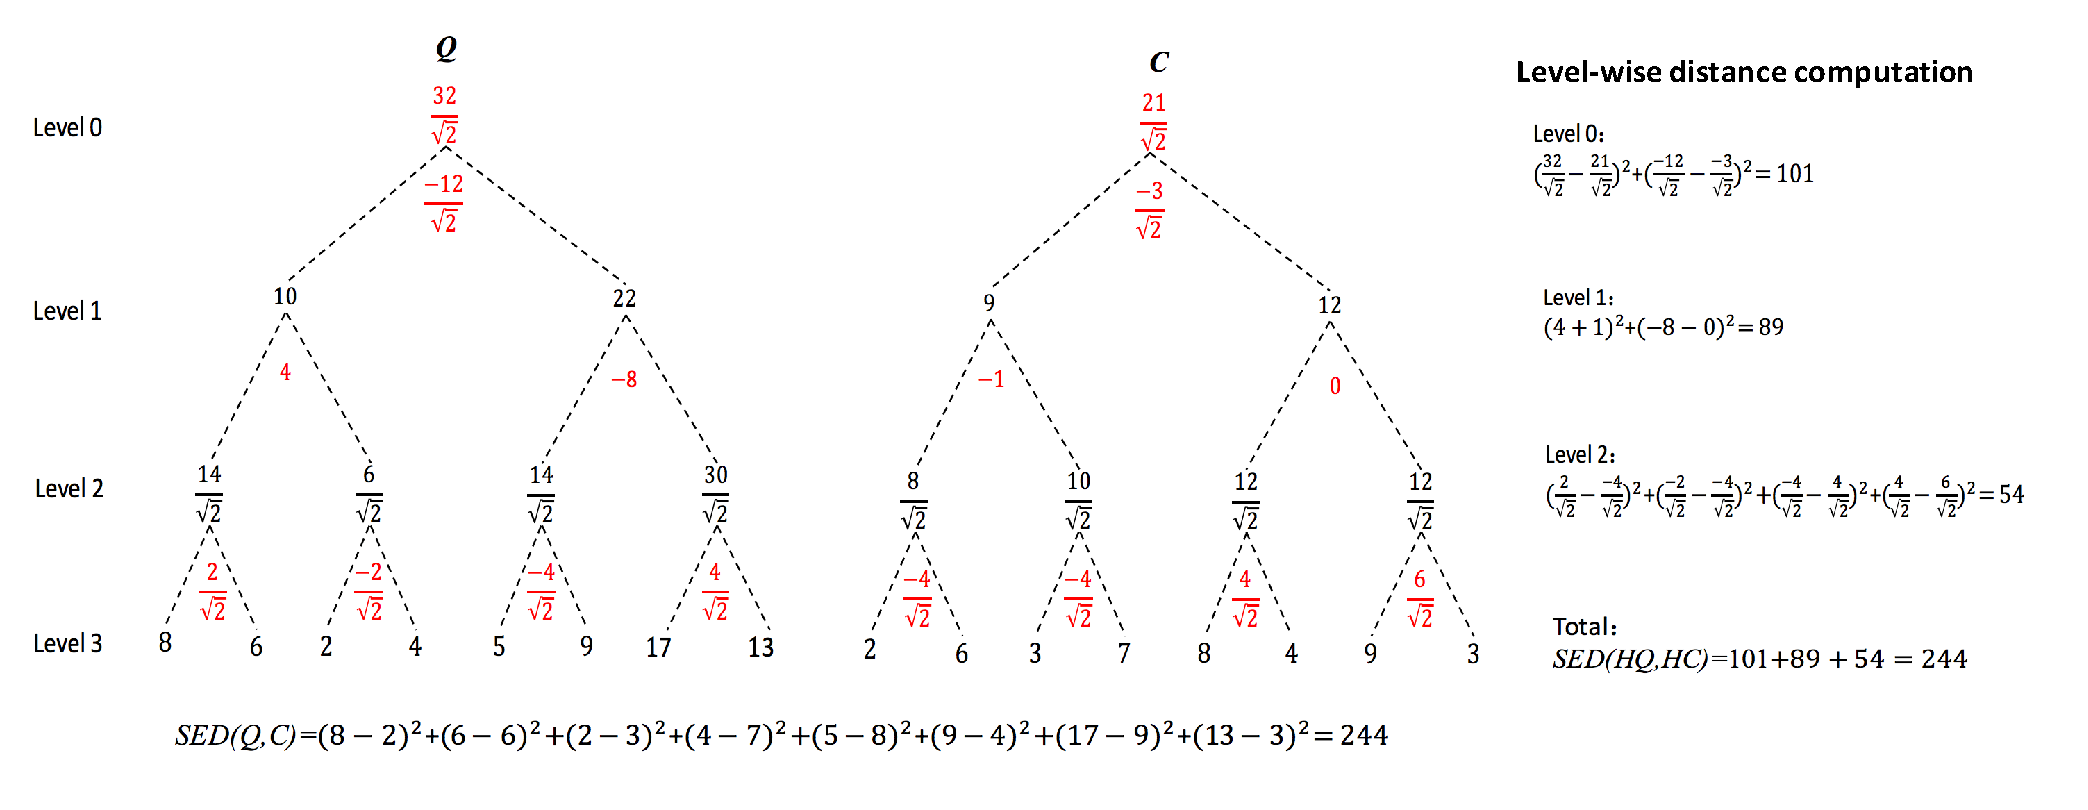
\includegraphics[width=0.95\textwidth]{Fig/chapter4/distance}
	\caption{基于Haar小波系数的距离计算示例}
	\label{fig-chapter4-distance}
\end{figure}

图\ref{fig-chapter4-distance}针对引理\ref{theory:dis}给出了示例说明。假定给定查询时间序列${\cal Q} = \{8, 6, 2, 4, 5, \\9, 17, 13\}$,
另一条序列为${\cal C}=\{2, 6, 3, 7, 8, 4, 9, 3\}$。通过计算可得,这两条序列间的欧式距离为$244$。接着,我们队这两条序列分别进行哈尔小波变换分别得到如图所示的两颗误差树。对每一层的系数进行欧式距离计算分别得到距离值101、89和54。其中第$0$层计算时把最终的均值也算进去了。通过计算发现系数的累加和确实等于原始序列的欧式距离。

\subsection{基于哈尔小波的欧式距离上、下界}
上一节介绍了,利用完整的哈尔小波系数,即全部的概要数据,能够用来计算原始的轨迹间欧式距离。但全部概要数据的数据量于原始轨迹数据量相同,不能达到降低通信开销的目的。为此
本节将介绍如何利用部分概要来计算轨迹的上、下界。首先根据引理\ref{theory:dis},我们有:
\begin{eqnarray}\label{eq:match}
SED({\cal Q},{\cal C}) &=& \sum\nolimits_{i=0}^{L-1}SED_{i}({\cal Q},{\cal C}) \nonumber\\ 
           &=&\sum\nolimits_{i=0}^{l}SED_{i}({\cal Q},{\cal C})+\sum\nolimits_{i=l+1}^{L-1}SED_{i}({\cal Q},{\cal C})
\end{eqnarray}

假设远程结点由粗到细已经获取了查询轨迹$\cal Q$的前$l+1$层概要数据,我们的目标就是根据这些已有的数据计算出$\cal Q$与任一候选$\cal C$的欧式距离上、下界。公式 \ref{eq:match}有半部分分为两部分,前半部分可以根据已有概要数据计算出来,后半部分无法直接计算。为此,我们将后半部分继续展开,得到如下:
\begin{eqnarray}\label{eq:decompose}
\sum_{i=l+1}^{L-1}SED_{i}({\cal Q},B)= \sum_{i=l+1}^{L-1}\sum_{j=0}^{2^i-1}(||\vd_{i,j}^{\cal Q}||^2+||\vd_{i,j}^{\cal C}||^2 -
2  \vd_{i,j}^{\cal Q} \bigcdot \vd_{i,j}^{\cal C}) 
\end{eqnarray}

公式\ref{eq:decompose}右半部分含有3个元素,第一个元素为查询轨迹$\cal Q$ 剩下概要数据的和, 该值可根据已有概要数据计算出来,计算方法为$SSQ-\sum_{i=0}^{l}\sum_{j=0}^{2^i-1}||\vd_{i,j}^{\cal Q}||^2$,其中$SSQ$为$\cal Q$所有系数的累加和。远程结点只需一开始就把$SSQ$发给所有远程结点即可。同理,第二个元素可在远程结点计算出来。难点在于对第三个关于系数內积累加和的计算。本文的做法是使用两次柯西—施瓦茨不等式估计其区间。第一次使用具体过程如下:
\begin{eqnarray}\label{eq:suofang1}
	-2\sum_{i=l+1}^{L-1}\sum_{j=0}^{2^i-1} ||\vd_{i,j}^{\cal Q}||\cdot ||\vd_{i,j}^{\cal C}||
	\le  \sum_{i=l+1}^{L-1}\sum_{j=0}^{2^i-1} -2\vd_{i,j}^{\cal Q}\bigcdot \vd_{i,j}^{\cal C} 
	\le  2\sum_{i=l+1}^{L-1}\sum_{j=0}^{2^i-1} ||\vd_{i,j}^{\cal Q}||\cdot ||\vd_{i,j}^{\cal C}||
\end{eqnarray}
接着我们对$\sum_{i=l+1}^{L-1}\sum_{j=0}^{2^i-1} ||\vd_{i,j}^{\cal Q}||\cdot ||\vd_{i,j}^{\cal C}||$进行再次使用柯西-施瓦茨不等式放缩:
\begin{eqnarray}\label{eq:suofang2}
\sum_{i=l+1}^{L-1}\sum_{j=0}^{2^i-1} ||\vd_{i,j}^{\cal Q}||\cdot ||\vd_{i,j}^{\cal C}|| \le 
	\sqrt{\sum_{i=l+1}^{L-1}\sum_{j=0}^{2^i-1}||\vd_{i,j}^{\cal Q}||^2} \cdot \sqrt{\sum_{i=l+1}^{L-1}\sum_{j=0}^{2^i-1}||\vd_{i,j}^{\cal C}||^2}
\end{eqnarray}
结合公式\ref{eq:suofang1}和\ref{eq:suofang2},我们得到如下完整的对$\sum_{i=l+1}^{L-1}\sum_{j=0}^{2^i-1} -2\vd_{i,j}^{\cal Q}\bigcdot \vd_{i,j}^{\cal C} $计算出如下上、下界。
 \begin{eqnarray}\label{eq:bound}
&&-2\sqrt{\sum_{i=l+1}^{L-1}\sum_{j=0}^{2^i-1}||\vd_{i,j}^{\cal Q}||^2} \cdot \sqrt{\sum_{i=l+1}^{L-1}\sum_{j=0}^{2^i-1}||\vd_{i,j}^{\cal C}||^2} \nonumber \\
&& 
\le  \sum_{i=l+1}^{L-1}\sum_{j=0}^{2^i-1} -2\vd_{i,j}^{\cal Q}\bigcdot \vd_{i,j}^{\cal C} 
\le  2\sqrt{\sum_{i=l+1}^{L-1}\sum_{j=0}^{2^i-1}||\vd_{i,j}^{\cal Q}||^2} \cdot \sqrt{\sum_{i=l+1}^{L-1}\sum_{j=0}^{2^i-1}||\vd_{i,j}^{\cal C}||^2}
\end{eqnarray}
最终,我们对欧式距离获得如下上、下界:
\allowdisplaybreaks
\begin{align} \label{eq:HaarBound}
&&	HLB_{l}({\cal Q},{\cal C}) =\sum_{i=0}^{l}SED_{i}({\cal Q},{\cal C})+
\sum_{i=l+1}^{L-1}\sum_{j=0}^{2^i-1}(||\vd_{i,j}^{\cal Q}||^2+||\vd_{i,j}^{\cal C}||^2)+ S_{0}({\cal Q},{\cal C}) \\
&&  - 2\sqrt{\sum_{i=l+1}^{L-1}\sum_{j=0}^{2^i-1}||\vd_{i,j}^{\cal Q}||^2} \cdot \sqrt{\sum_{i=l+1}^{L-1}\sum_{j=0}^{2^i-1}||\vd_{i,j}^{\cal C}||^2} \nonumber \\
&&	HUB_{l}({\cal Q},{\cal C}) = \sum_{i=0}^{l}SED_{i}({\cal Q},{\cal C})+
\sum_{i=l+1}^{L-1}\sum_{j=0}^{2^i-1}(||\vd_{i,j}^{\cal Q}||^2+||\vd_{i,j}^{\cal C}||^2)+S_{0}({\cal Q},{\cal C}) 
\nonumber \\
&&\qquad \quad + 2\sqrt{\sum_{i=l+1}^{L-1}\sum_{j=0}^{2^i-1}||\vd_{i,j}^{\cal Q}||^2} \cdot \sqrt{\sum_{i=l+1}^{L-1}\sum_{j=0}^{2^i-1}||\vd_{i,j}^{\cal C}||^2}
\end{align}
\allowdisplaybreaks[4]

进一步的我们提出两个性质,这两个性质表明我们的上、下界会随着概要数据的增加而越来越紧。它们的证明过程见本章附件。
\begin{theorem}[]\label{theory:lower}
	$HLB$会随着粒度的概要数据粒度的增加而逐渐上升,即$HLB_{l} \le HLB_{l+1}$。
	%The lower bound $HLB$  is non-decreasing when we move from level $l$ to ${l+1}$, i.e., $HLB_{l} \le HLB_{l+1}$.
\end{theorem}

\begin{theorem}[]\label{theory:upper}
	$HUB$会随着粒度的概要数据粒度的增加而逐渐下降,即$HUB_{l} \ge HUB_{l+1}$。
%	The upper bound $HUB$ is non-increasing when we move from level $l$ to  ${l+1}$, i.e., $HUB_{l} \ge HUB_{l+1}$.
\end{theorem}

\begin{figure}
	\centering
	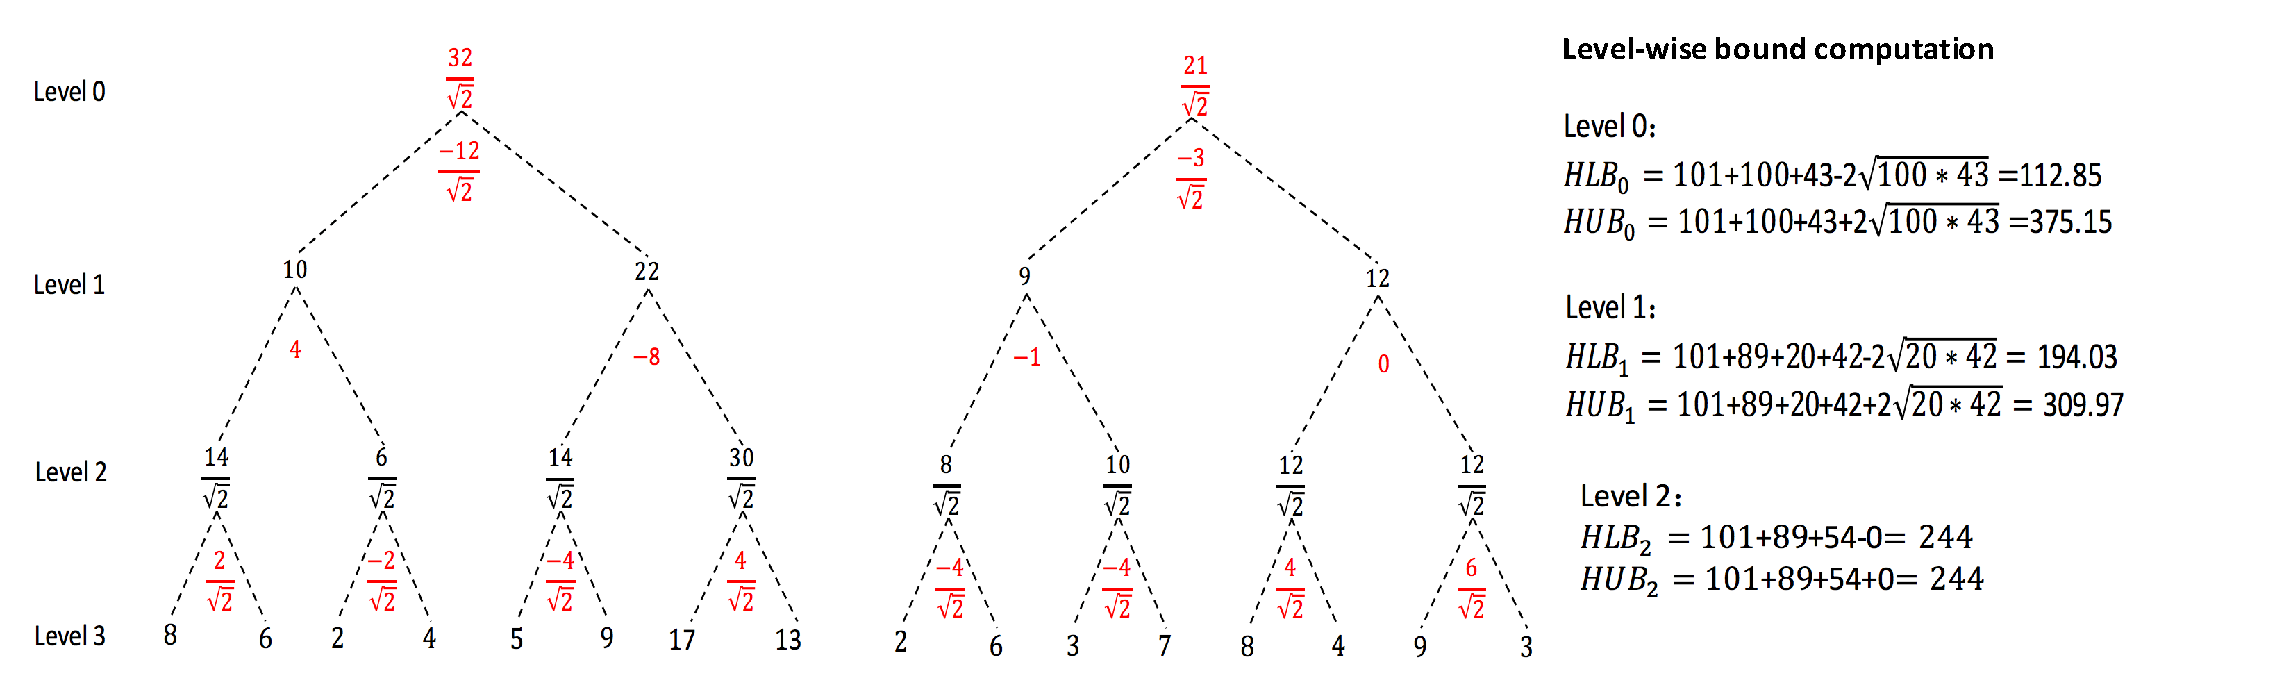
\includegraphics[width=0.95\textwidth]{Fig/chapter4/bound}
	\caption{欧式距离上、下界示例}
	\label{fig-chapter4-bound}
\end{figure}

图\ref{fig-chapter4-bound}介绍了使用概要数据得到越来越紧的上、下界,并直至逼近到真实距离的过程。其使用的数据与图\ref{fig-chapter4-distance}一样。当查询对象的第$0$层系数(数据量为1)发送给远程结点后,远程结点可以对其局部时间序列$\cal C$根据公式\ref{eq:HaarBound},计算得到上界和下界分别为$375.15$和$112.85$。当第$1$层系数(数据量为2)发过去后得到更紧的上界和下界分别为$309.97$和$194.03$。当第$2$层系数(即最后一层)发过去后,可以发现此时的上、下界等于真实的距离值。

 \section{基于欧式距离的查询算法:ED-FTB}\label{sec-c4-algorithm}
 \subsection{ED-FTB算法实现}
\begin{algorithm}[t]
	\renewcommand{\baselinestretch}{1}
	\caption{{\sl ED-FTB}\label{alg:EDCoordinator}在协调者结点}
	\begin{algorithmic}[2]
		\STATE /* \emph{ED-FTB协调者结点函数接口实现} */
	\end{algorithmic}
	\textbf{coordinatorInit}(${\cal Q} ,  {\cal R}$)
	\begin{algorithmic}[1]
		\STATE  $l\leftarrow -1$;
		\STATE $HQ \leftarrow$ Haar wavelet coefficients of $\cal Q$;\COMMENT{待查询轨迹获取哈尔小波系数}
		\STATE $SSQ = \sum_{i=0}^{n-1}||HQ_{i}||^2$;\COMMENT{所有系数的平方和}
		%		\STATE $l\leftarrow -1$;
		\STATE 	\textsf{sendToRemoteSites}(${\cal R}$, $SSQ$);
	\end{algorithmic}
	
	\textbf{generateInfo()}
	\begin{algorithmic}[1]
		\STATE $l\leftarrow l+1$;
		\STATE return $\widehat {\cal Q}_{l}$;\COMMENT{返回第$l$层哈尔小波系数}
	\end{algorithmic}
\end{algorithm}

\begin{algorithm}[t]
	\renewcommand{\baselinestretch}{1}
	\caption{{\sl ED-FTB}\label{alg:EDRemote}在远程结点}
	\begin{algorithmic}[2]
		\STATE /* \emph{ED-FTB远程结点函数接口实现} */
	\end{algorithmic}
	
	\textbf{remoteInit($TS_{r} , S_{r}$)}
	\begin{algorithmic}[1]
		\IF{第一次接受查询}
		\FORALL{ $\cal C$ in $TS_{r}$}
		\STATE $HC \leftarrow$ Haar wavelet coefficients of $\cal C$; \COMMENT{候选轨迹获取哈尔小波系数}
		\STATE $SSC = \sum_{i=0}^{n-1}||HQ_{i}||^2$;\COMMENT{所有系数的平方和}	   
		\ENDFOR
		\ENDIF
		\FORALL{ $\cal C$ in $TS_{r}$}
		\STATE $C\_BF \leftarrow  \langle 0,\infty \rangle$; \COMMENT {为$\cal C$初始化界特征}
		\STATE $S_{r}=S_{r} \cup C\_BF$;
		\ENDFOR
		\STATE $SSQ \leftarrow$\textsf{getFromCoordinator}();
	\end{algorithmic}
	
	\textbf{updateBounds}($S_{r}$, $M$) //边更新界边剪枝。
	\begin{algorithmic}[1]
		\FORALL{ $\cal C$ in $TS_{r}$}
		\STATE  $a=\sum_{i=l+1}^{L-1}\sum_{j=0}^{2^i-1}||\vd_{i,j}^{\cal Q}||^2$;$b=\sum_{i=l+1}^{L-1}\sum_{j=0}^{2^i-1}||\vd_{i,j}^{\cal C}||^2$;
		\STATE $tmp=a+b+S_{0}(\cal Q, \cal C)$;
		\STATE $lb=tmp -2\sqrt{ab}$;$ub=tmp+2\sqrt{ab}$;
		\IF{$ lb<gkub \quad \&\& \quad  (lb=lb+ \sum_{0}^{l}SED_{i}({\cal Q},{\cal C}))<gkub$}
		\STATE 将轨迹$\cal C$的界特征的下界更新为$lb$;
		\IF{$ub<gkub \quad \&\& \quad (ub=ub+ \sum_{0}^{l}SED_{i}({\cal Q}, {\cal C}))<gkub)$}
		\STATE $ ub=ub+ \sum_{0}^{l}SED_{i}({\cal Q}, {\cal C})$;
		\STATE 将轨迹$\cal C$的界特征的上界更新为$ub$;
		\ENDIF
		\ELSE
		\STATE 将该轨迹从$S_{r}$中移除;
		\ENDIF
		\ENDFOR
	\end{algorithmic}
\end{algorithm}

在上一节,我们已经利用概要数据提出了欧氏距离的上、下界。这使得在FTB框架中插入欧式距离成为可能。本节将详细介绍将欧式距离跟FTB相结合的查询算法ED-FTB。ED-FTB维持了FTB框架的主要结构,只对本章第一节所介绍的接口进行了具体实现。

算法\ref{alg:EDCoordinator}介绍了协调者节点的上的函数接口的实现方法。在\textsf{coordinatorInit}函数中,我们对待查询轨迹进行哈尔小波变换,并计算出其所有系数的平方和。接着将该平方和发送给所有远程结点。远程结点在将来将会利用该值进行上、下界计算。
由于FTB框架是迭代式由粗到细的通信计算框架,在每轮的迭代中会将某一层的概要数据(哈尔小波系数)发送给远程结点。因此,在初始化过程中我们用$l$来记录当前已经发送到哪一层的数据,并将$l$初始化为$-1$以便从第0层开始。此外,我们在\textsf{generateInfo}中准备将要发送的下一层概要数据,以便协调者结点发送。

接着,算法\ref{alg:EDRemote}介绍运行在远程结点的函数。对于\textsf{RemoteInit}函数,若远程结点是第一次接受查询,则会为每条候选轨迹进行哈尔小波变换并计算系数的平方和。若不是,则为该结点所包含的每条轨迹初始化界特征信息(下界初始化为0,上界初始化为正无穷),并接受查询轨迹的系数平方和。在查询执行过程中\textsf{UpdateBounds}函数为候选更新上、下界。直接实现方式为根据上、下界的计算公式,计算出这两个值。但由于查询过程中的主要计算开销就是对所有候选更新界特征。所以,降低该过程的计算开销很有必要。

为降低更新界特征的计算开销,本文引入了在更新界过程中进行剪枝的思想。在介绍此方法前,我们再次回顾下我们的下界。我们的下界计算主要包含3个算子:首先是$\sum_{i=0}^{l}SED_{i}({\cal Q},{\cal C})$,其计算复杂度为O($2^{l}$)。其次是$\sum_{i=l+1}^{L-1}\sum_{j=0}^{2^i-1}||\vd_{i,j}^{\cal Q}||^2$,由于该部分可以通过$SSQ-\sum_{i=0}^{l}\sum_{j=0}^{2^i-1}||\vd_{i,j}^{\cal Q}||^2$计算,而且$\sum_{i=0}^{l-1}\sum_{j=0}^{2^i-1}||\vd_{i,j}^{\cal Q}||^2$的值已知。故该部分的计算复杂度也为$O(2^{l})$。同理,第三部分$\sum_{i=l+1}^{L-1}\sum_{j=0}^{2^i-1}||\vd_{i,j}^{\cal C}||^2$计算复杂度也为$O(2^{l})$。除这三个算子的计算法外,剩余部分的计算复杂度为$O(1)$。

基于以上分析。假设我们已知若轨迹下界值超过$\alpha$,那该条轨迹即不可能称为候选。此时,我们可以在更新下界的同时进行剪枝(算法\ref{alg:EDRemote}:\textsf{UpdateBounds}函数)。具体的做法是我们首先计算出第二和第三两个算子,并根据这两个算子的值计算出下界中除$\sum_{i=0}^{l}SED_{i}({\cal Q},{\cal C})$以外部分的值。若此时计算出来的值已超过$gkub$,则无需继续求解下界和上界,直接将该候选删除。若仍小于$gkub$,则计算出完整的下界,并判断此时下界值是否小于$gkub$,若小于则停止计算上界并将该候选删除。当更新完下界后,我们先计算出上界中除$\sum_{i=0}^{l}SED_{i}({\cal Q},{\cal C})$以外部分的值。若该部分值超过$gkub$,则该轨迹的上界对选取新一轮的全局最小的$k$个上界没有帮助,无需计算该轨迹的具体上界值。否则,计算出具体的上界并更新界特征。此时,需要注意的是,在FTB框架算法的第7-9行中,我们仅需传递上界小于 $gkub$的$k$个最小上界。若个数不足$k$个,则只传递满足$gkub$的上界。
 
 \subsection{ED-FTB算法性能分析}
 在分析前,我们先介绍对比算法LEEWAVE-CL。LEEWAVE-CL是在LEEWAVE算法的基础上使用了本文所提下界(比原始的下界更紧)。LEEWAVE-CL算法也是迭代式算法。在它的每次迭代中,远程结点根据获取的概要数据,为每个候选计算如下两个算子:$\sqrt{\sum_{i=l+1}^{L-1}\sum_{j=0}^{2^i-1}||\vd_{i,j}^{\cal C}||^2}$ 和  $S_{0}({\cal Q},{\cal C})+\sum_{i=0}^{l}SED_{i}({\cal Q},{\cal C})$。然后协调者节点获取者些参数并为每个候选计算上、下界,并利用界特征进行过滤。然后,将候选列表发给对应远程结点。LEEWAVE-CL方法与本文方法的最大不同就是,它在协这结点进行界特征的计算和过滤,而ED-FTB是在所有远程结点进行。接下来,我们将从时间和通信两个方面对ED-FTB和LEEWAVE-CL进行对比分析。在此之前,我们使用如下标记:(i)使用$|C_{i}|$ 和 $|CS_{i}|$ 分别表示第$i$($i\ge 0$)次迭代前候选轨迹的数量和包含候选轨迹的远程结点数量。由于采用相同的上、下界,这两个算法的迭代次数相同,我们假定迭代次数为$\lambda$($\lambda \le \log_{2}n$)。
 
  \textbf{时间复杂度:}不考虑系统初始化时对所有候选进行哈尔小波变换的时间开销, ED-FTB和LEEWAVE-CL两者的时间开销来自迭代式计算时更新上、下界,所以他们的时间复杂度一样。计算复杂度最坏的情况就是所有候选都集中在一个结点上,则更新上、下界的时间复杂度为$O(\sum_{i=0}^{\lambda-1} d\cdot |C_{i}| \cdot 2^{i})$。此外,由于$k$值一般较小,算法运行过程中涉及到的查找局部最小的$k$个上界耗时较低,可以忽略。总的来说,ED-FTB和LEEWAVE-CL的时间复杂度均为$O(\sum_{i=0}^{\lambda-1} d\cdot |C_{i}| \cdot 2^{i})$。但ED-FTB由于在各个结点进行界特征的计算,且采用了边计算边过滤的策略,故其实际计算开销低于LEEWAVE-CL。
 
  \textbf{通信复杂度:}
ED-FTB和LEEWAVE-CL的通信开销主要集中在迭代式计算过程中。ED-FTB在第$i$轮迭代时,需要花费$O(d\cdot 2^{i}\cdot |CS_{i}|+|C_{i}|)$ 代价以将第$i$层概要数据发送给候选结点,并至多接收$|C_{i}|$个上界(用于计算全局的剪枝阈值)。在$\lambda$次迭代后,总的通信开销为$O(\sum_{i=0}^{\lambda-1}(d \cdot 2^{i} \cdot|CS_{i}| + |C_{i}|))$。
LEEWAVE-CL 在第$i$轮迭代需要花费 $O(|CS_{i}| \cdot (d\cdot 2^{i}+ |C_{i+1}|))$ 来讲概要数据和所有候选的列表发送给所有候选结点。此外,还需要花费$O(d\cdot |C_{i+1}|)$代价以接受每个候选轨迹的两个算子值以便在协调者结点计算出上、下界。所以,当$\lambda$次迭代后,其总的通信开销为$O(|CS_{i}| \cdot (d\cdot 2^{i}+ |C_{i+1}|)+d\cdot |C_{i+1}|)$。对比两个算法的开销值,我们可以发现ED-FTB的能节省更多通信开销。
 
 \section{实验分析}\label{sec-c4-Exp}
本节将在真实世界的轨迹数据上评估本章节所提出的算法。本小节首先介绍使用的真实世界轨迹数据集及实验设置。接着从分别验证了算法的有效性和可扩展性。

\subsection{实验设置}
本章工作在实验中使用北京出租车数据集,该数据集已被广泛应用于轨迹数据分析。该数据集采集了北京市三万多辆出租车在2013年10月份到12月份三个月内的行驶GPS轨迹。每个GPS轨迹点包含的数据维度较多,我们仅选取了位置(经度和纬度)、时间、速度和角度这五个维度的值,并进行了归一化预处理。我们从该数据集中截取了两个子数据集:\emph{T-Small}和\emph{T-Big}以分别验证算法的有效性和可扩展性。
\emph{T-Small}截取了10月1至7号间 上午8点到10点的轨迹数据,并从中选出最长的1万条轨迹进行分析。
\emph{T-Big} 截取了11月1号至12月31号间每天上午8至10点和下午5至7点两个时间段的1百万条轨迹数据。为满足实验需求,这两个数据集的每条轨迹长度均超过4,096。

在本章的实验中,我们将比较ED-FTB和LEEWAVE-CL算法的性能。LEEWAVE-CL算法在已有LEEWAVE算法的基础上使用了本文所提供的下界。
两个算法均用JAVA实现,并运行在一个包含12个结点的Spark集群上。每个结点包含8核因特尔E5335 2.0 GHz中央处理器和16GB的内存。我们在\emph{T-Small}数据集上验证了算法的有效性,在\emph{T-Big} 数据集上验证了算法的可扩展性。
%All codes, written in Java, were evaluated on a 12-node clustering running Spark 1.5.2 over Ubuntu 12.0.4. Each node is equipped with an 8 cores Intel E5335 2.0GHz processor and 16GB memory.
%contains 1,000,000 trajectories from November 1st to December 31st during 8:00 to 10:00 am and 17:00-19:00 pm.
%每个轨迹点包含的数据维度较多,我们仅选取了位置(经度和纬度)、时间、速度和角度这五个维度的值,并进行了归一化预处理。


\subsection{算法有效性}

\begin{figure}[t]
	\centering
		\centering
		\subfigure[$k=1$]{
			\label{fig:EDpruk1}
			\includegraphics[width=2.7in]{Fig/chapter4/EDpruk1.eps}
		}
		\subfigure[$k=10$]{
			\label{fig:EDpruk10}
			\includegraphics[width=2.7in]{Fig/chapter4/EDpruk10.eps}
		}
	\\
		\subfigure[$k=50$]{
		\label{fig:EDpruk50}
		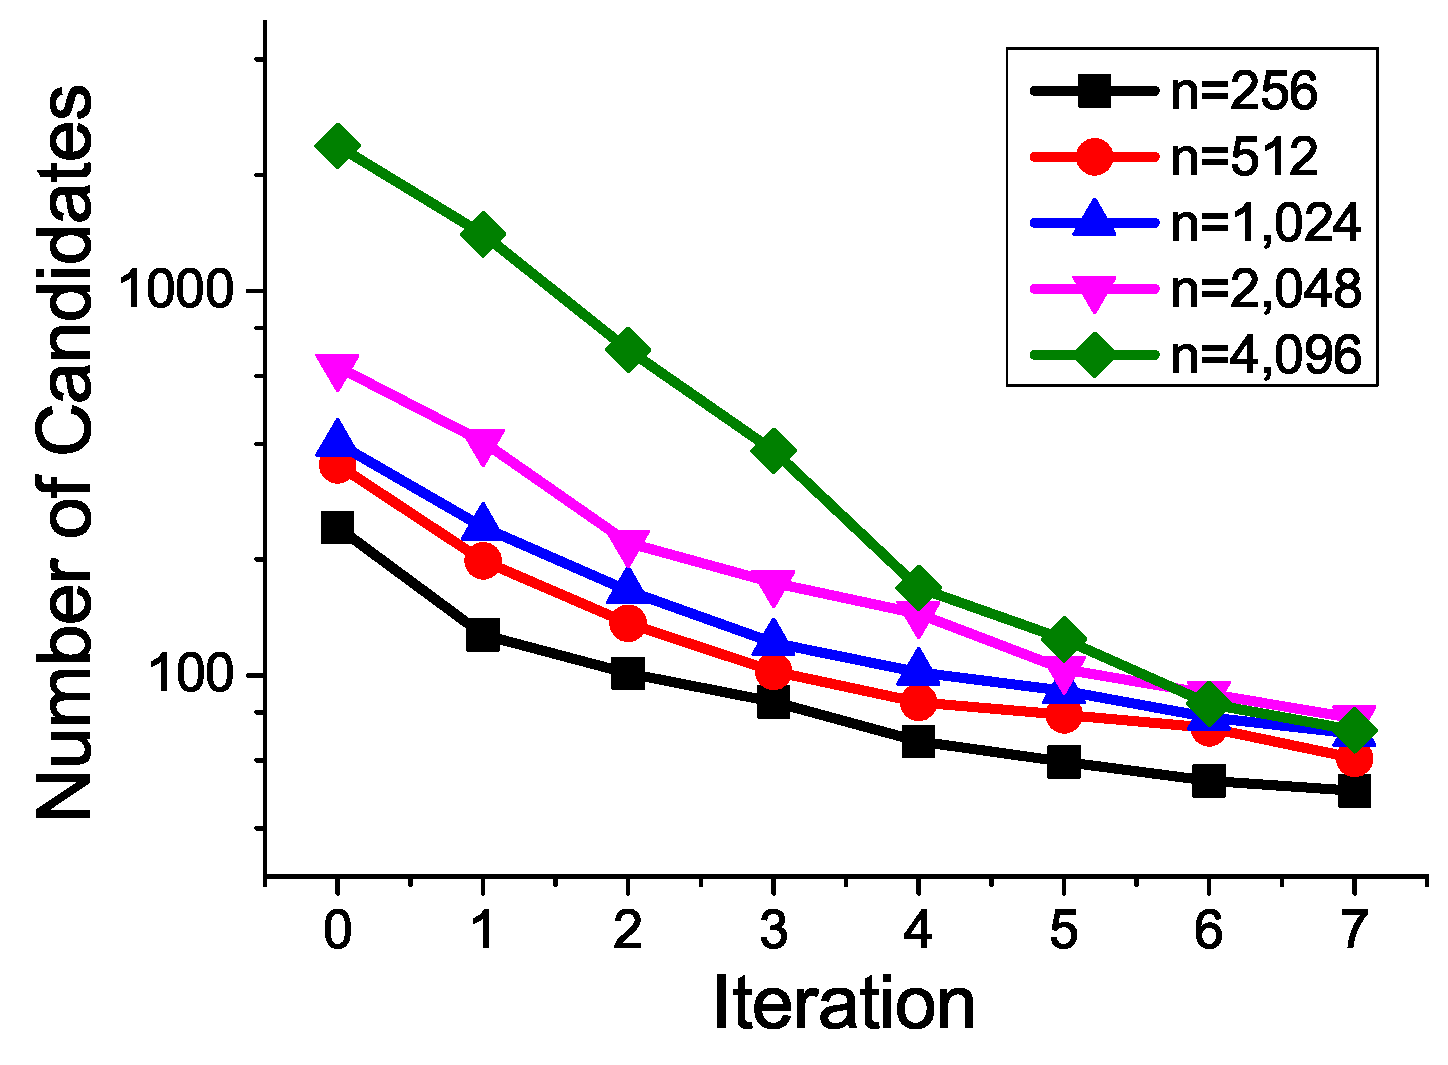
\includegraphics[width=2.7in]{Fig/chapter4/EDpruk50.eps}
		}
		\subfigure[$k=100$]{
			\label{fig:EDpruk100}
			\includegraphics[width=2.7in]{Fig/chapter4/EDpruk100.eps}
		}
		\caption{ED-FTB剪枝效果图}
		\label{fig:ED-DTKTS}
\end{figure}
首先,我们通过观察迭代过程中每轮结束后的剩余候选数来研究ED-FTB算法的剪枝效果。在该组实验中,我们将$M$设置为10,000,并研究了不同长度轨迹剪枝的效果。图 \ref{fig:ED-DTKTS} 介绍了前8轮迭代中每轮迭代后的候选数。我们可以看出候选数在前5轮迭代中下降的较快且已经过滤掉绝大多数候选。这说明了我们的上、下界收敛速度较快,具有较好的剪枝效果。此外,我们可以发现短轨迹在前几轮中候选数下降的比长轨迹快。这是由于相同数据量的概要数据下短轨迹比长轨迹包含更多的原始轨迹的信息。最后,对比不同的 $k$值,我们发现$k$值越小,每轮所剩候选数越少。即$k$越小,剪枝效果越好。这是由于$k$值越小,我们所获得的全局第$k$小上界值就越小。而无论$k$值如何选取,每个候选的下界值不变。因此,越小的全局上界能通过下界剪枝掉更多的候选。同时,由于实际应用中$k$值通常都是一个很小的数。因而我们的算法能往往取得较好的效果。
\begin{figure}
		\centering
	\subfigure[$k=1$]{
		\label{fig:EDprucmpk1}
		\includegraphics[width=2.7in]{Fig/chapter4/cmp1.eps}
	}
	\subfigure[$k=10$]{
		\label{fig:EDprucmpk10}
		\includegraphics[width=2.7in]{Fig/chapter4/cmp10.eps}
	}
\\
	\subfigure[$k=50$]{
		\label{fig:EDprucmpk50}
		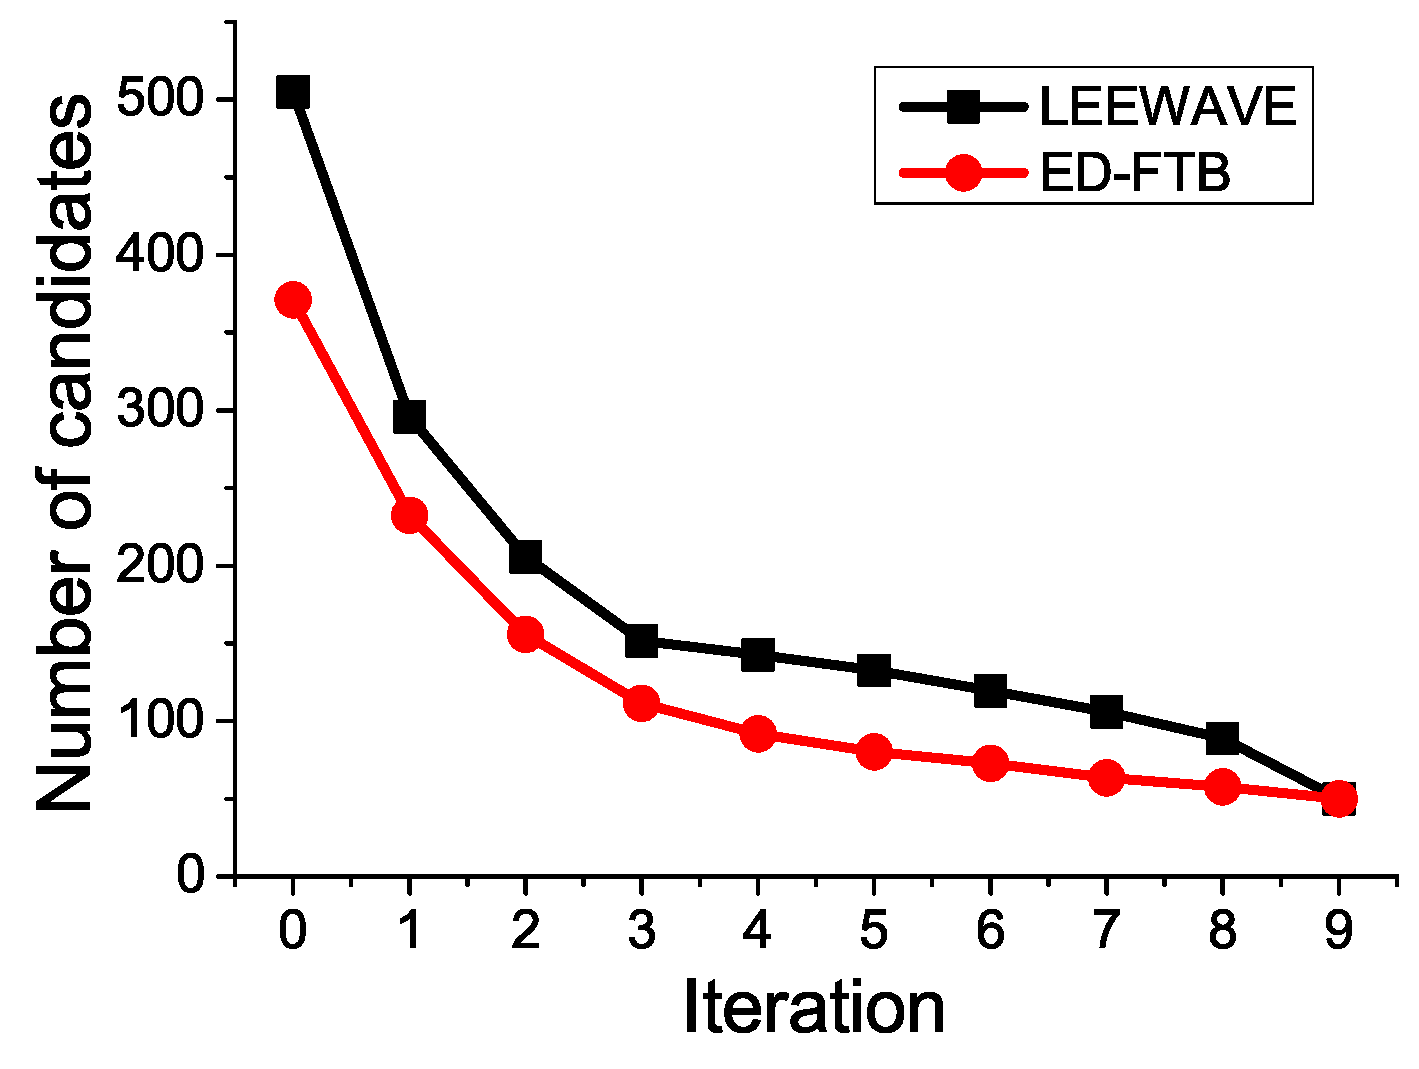
\includegraphics[width=2.7in]{Fig/chapter4/cmp50.eps}
	}
	\subfigure[$k=100$]{
		\label{fig:EDprucmpk100}
		\includegraphics[width=2.7in]{Fig/chapter4/cmp100.eps}
	}
	\caption{下界对剪枝结果的影响}
	\label{fig:PruningCmp}
\end{figure}

然后,我们对比研究了ED-FTB的剪枝效果和ED-FTB使用LEEWAVE中的下界后的剪枝效果,以分析下界对剪枝效果的影响。
在该组实验中,我们将$M$值设置为10,000,轨迹长度设为$1,024$。图\ref{fig:PruningCmp}对比展示了不同$k$值下,不同下界对剪枝的影响。其中LEEWAVE代表ED-FTB算法使用LEEWAVE算法中的下界后的结果。从图中,我们可以看出由于本文所提出的下界比已有算法的下界更紧,导致每轮迭代结束后ED-FTB所剩的候选数更少。这说明了本文所提下界的优越性。此外我们可以发现$k$值越小,两条曲线间的间隔越大。更能说明本文下界所取得的优越性越明显。


\begin{figure} [t]
	\centering
	\subfigure[$M=50,k=1$]{
		\label{50-1}
		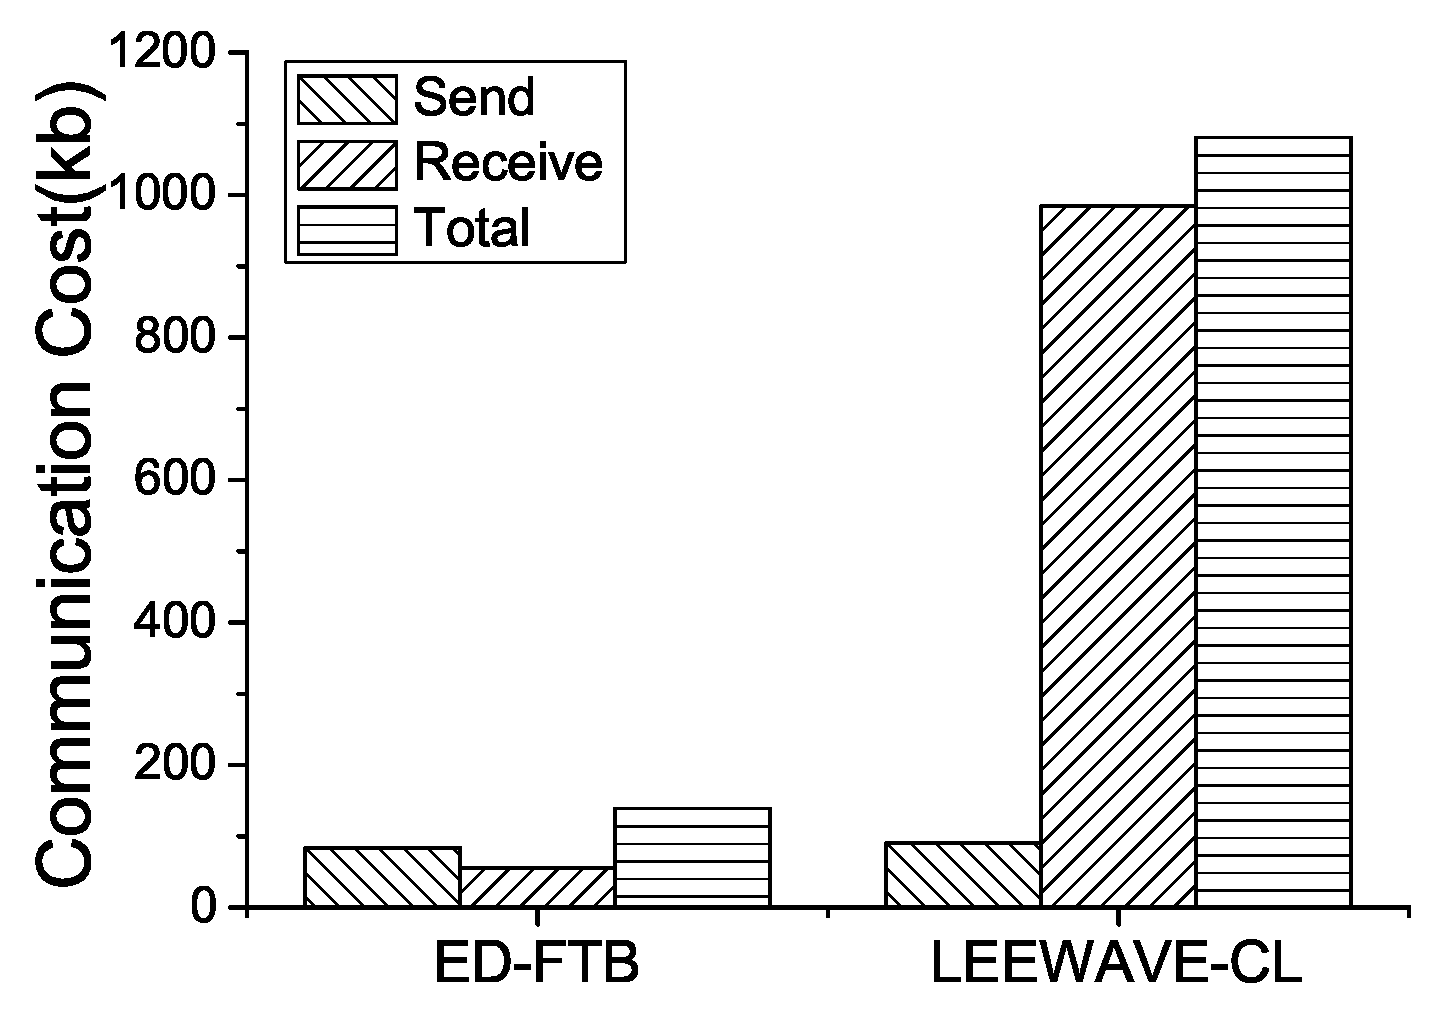
\includegraphics[width=2.7in]{Fig/chapter4/1k50m.eps}
	}
	\subfigure[$M=50,k=1,000$]{
		\label{50-1000}
		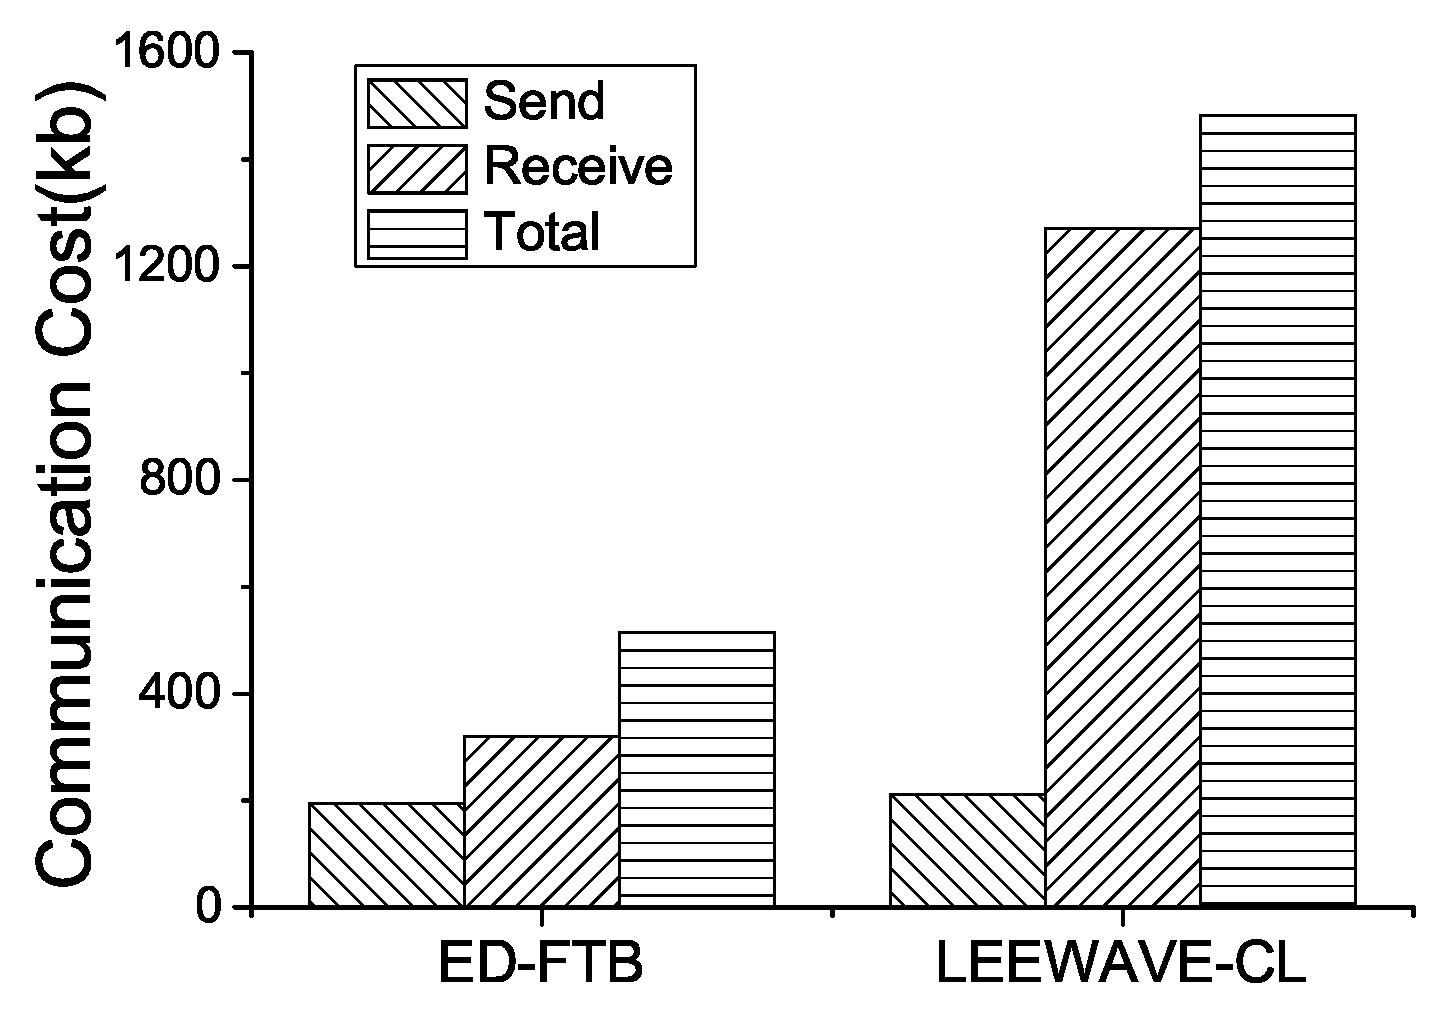
\includegraphics[width=2.7in]{Fig/chapter4/1000k50m.eps}
	}
	
	\subfigure[$M=200,k=1$]{
		\label{200-1}
		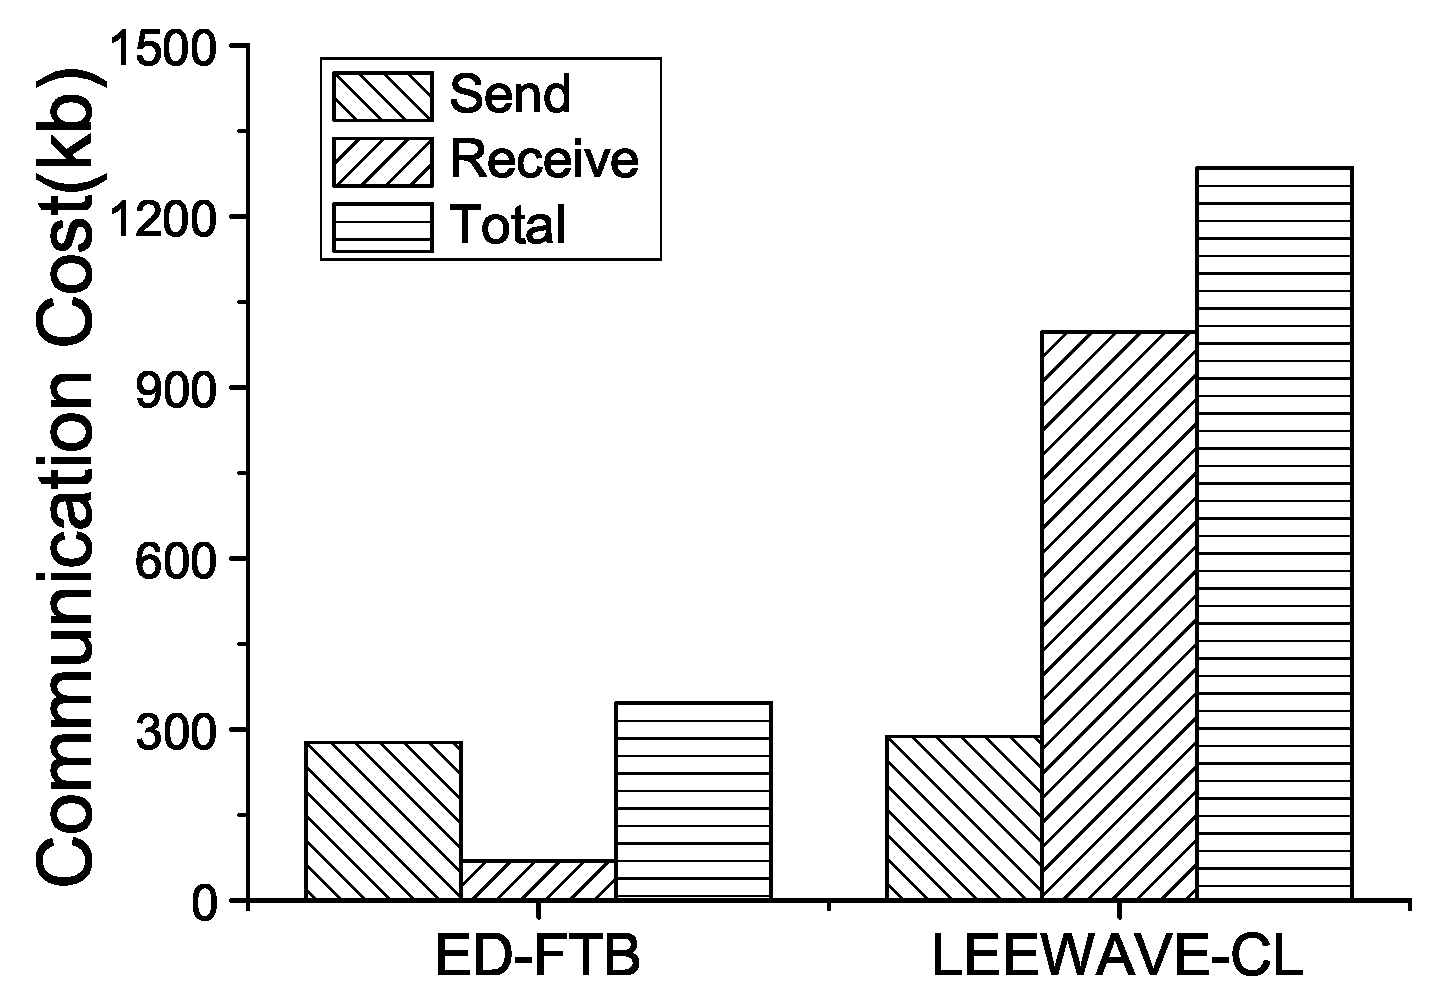
\includegraphics[width=2.7in]{Fig/chapter4/1k200m.eps}
	}
	\subfigure[$M=200,k=1,000$]{
		\label{200-1000}
		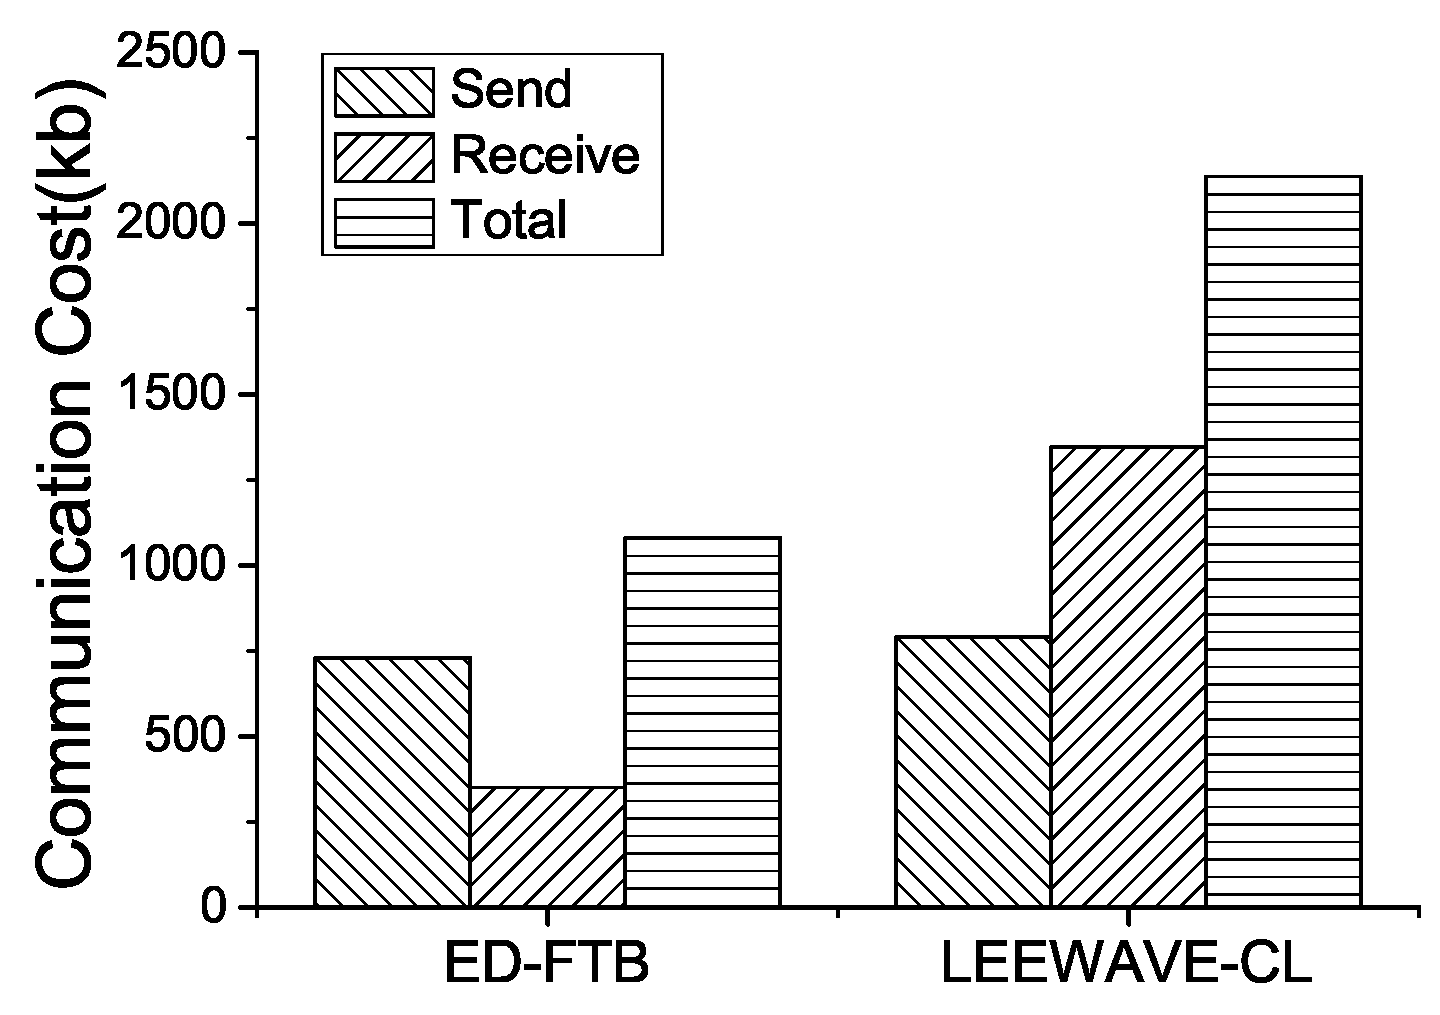
\includegraphics[width=2.7in]{Fig/chapter4/1000k200m.eps}
	}
	\vspace{-10pt}
	\caption{算法执行策略详细比较}
	\label{fig:components}
	\vspace{-0.5cm}
\end{figure}
接着,我们使用相同的界,对比了分析了本文所提查询策略与LEEWAVE所用查询策略对通信性能的影响。我们从协调者节点出发,研究了两种策略下它发送和接受的数据量以及总的数据通信开销。
图 \ref{fig:components}介绍了当$M$取50和$100$,k取$1$和$1000$下的实验结果。图中LEEWAVE-CL代表
结合了LEEWAVE的查询策略与本文的界特征后的算法。
从图中我们可以发现,协调者结点在两种策略下,发送的数据量差别不大且都比较小。这是因为,两个策略都有减少协调者数据发送的数据量这一共同目标。且两者使用的使用概要数据剪枝的策略很好的达成了这一目标。
但接受的数据量在两种策略下差别很大。ED-FTB所用的查询策略是在每个远程结点剪枝数据。每轮迭代完后远程结点仅需将所计算出来的局部最小的$k$个上界返回。而LEEAVE-CL需要将所有候选的跟计算界信息的两个算子返回。当远程结点所包含的数据越多,则两者的区别越大。特别地,当$k$值较小时(图 \ref{50-1} 和 \ref{200-1}),ED-FTB所收到的数据不到LEEWAVE-CL的十分之一。
%Especially, when $k$ is small(in Fig. \ref{50-1} and \ref{200-1}), the amount of data received in DT-KST is $10\%$ less than that of LEEWAVE-CL. 


\begin{figure}[t]
	\centering
		\centering
		\subfigure[$M=100$]{
			\label{fig:costM100}
			\includegraphics[width=2.7in]{Fig/chapter4/costM100.eps}
		}
		\subfigure[$M=1,000$]{
			\label{fig:costM1000}
			\includegraphics[width=2.7in]{Fig/chapter4/costM1000.eps}
		}
	\\
		\subfigure[$M=5,000$]{
		\label{fig:costM5000}
		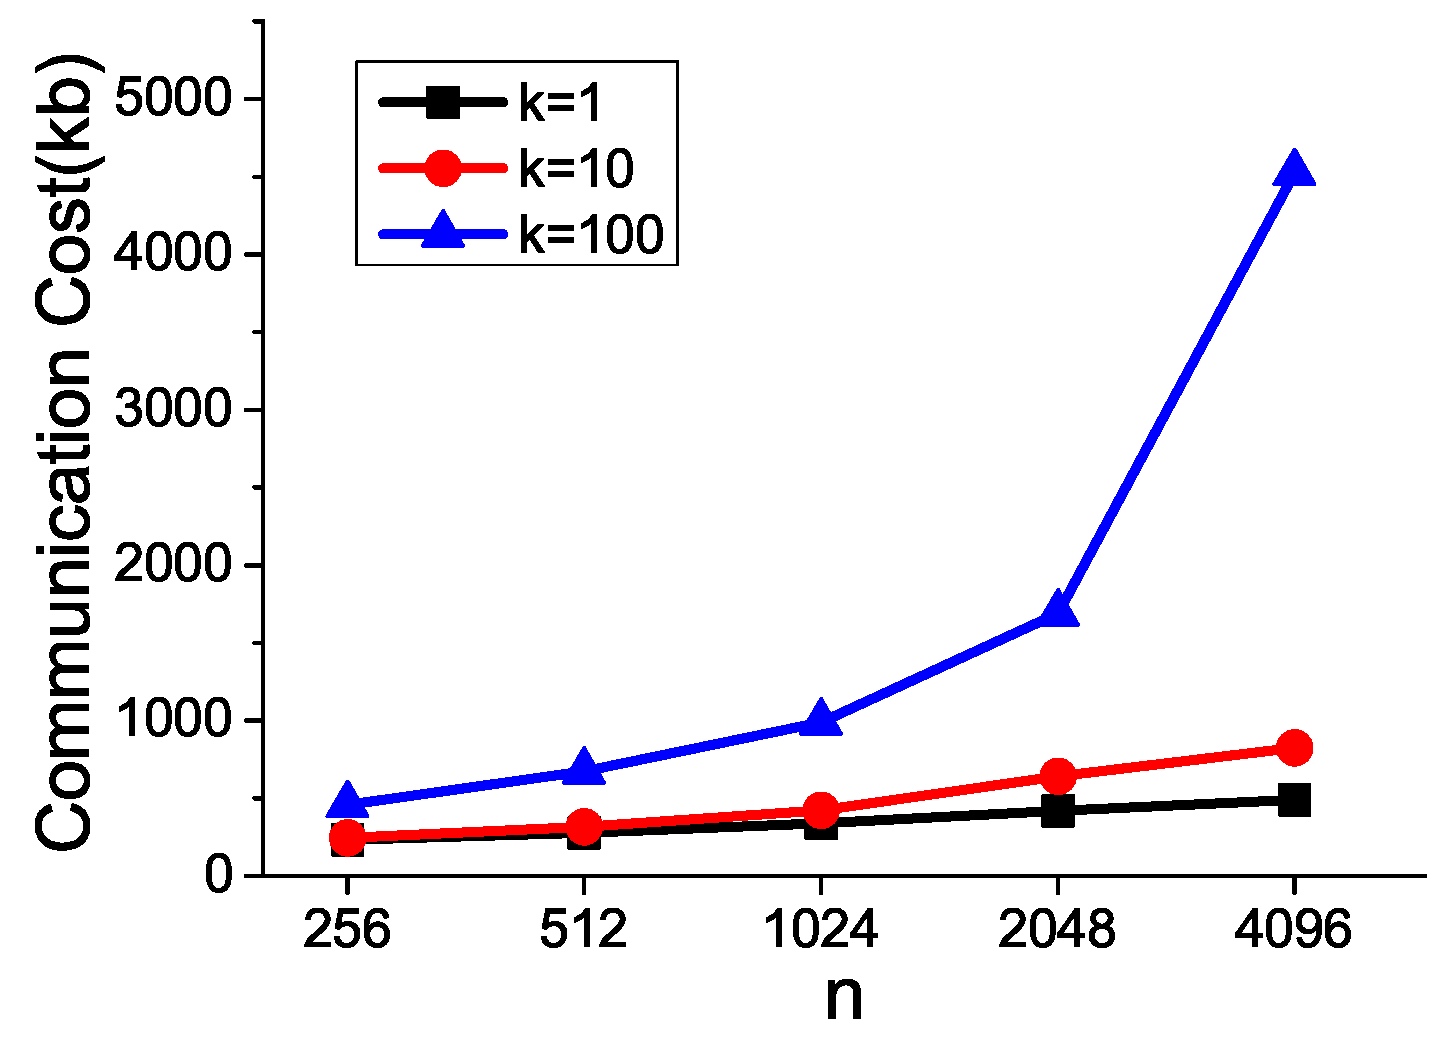
\includegraphics[width=2.7in]{Fig/chapter4/costM5000.eps}
	}
		\subfigure[$M=10,000$]{
			\label{fig:costM10000}
			\includegraphics[width=2.7in]{Fig/chapter4/costM10000.eps}
		}
		\caption{$n$,$k$和$M$对ED-FTB算法通信开销的影响}
		\label{fig:costKM}
\end{figure}
其次,我们研究了$n$,$k$和$M$对ED-FTB算法通信开销的影响。在该组实验中,我们将$n$的值从256变化到$4,096$,将$k$的值从1变化到100。图\ref{fig:costKM}展示了不同$M$值下($M$从100编化到$10,000$),ED-FTB算法通信开销随参数变化的结果。首先,我们看出随着$k$值的增加,通信开销逐步增加。这是由于$k$值越大,每轮所剩候选数越多,候选所在的远程结点也就越多。从而每轮需要将概要数据发送到更多的候选结点中。其次,随着$n$值的增加通信开销也在增加。这是由于长轨迹需要发送更多的数据才能达到与短轨迹相同的剪枝效果。最后,对比三幅图可以发现,随着远程结点数据的增加,通信开销也在增加。这是由于在每轮迭代中,远程结点增加后,候选轨迹会分布到更多的结点中。因而,算法需要将概要数据发送到更多的结点中。因而总的通信开销也会增加。但是,对于极端情况$M=10,000$时,此时每个远程结点仅包含一条轨迹时我们的通信开销仍不到$10$Mb,远小于直接方法的开销(约$640$Mb)。因此,ED-FTB算法具有较高的通信节约性能。

\begin{figure}[t]
\centering
\subfigure[$k=1$]{
	\label{fig:costCmpk1}
	\includegraphics[width=2.7in]{Fig/chapter4/cmpk1.eps}
}
\subfigure[$k=10$]{
	\label{fig:costCmpk10}
	\includegraphics[width=2.7in]{Fig/chapter4/cmpk10.eps}
}
\\
\subfigure[$k=50$]{
	\label{fig:costCmpk50}
	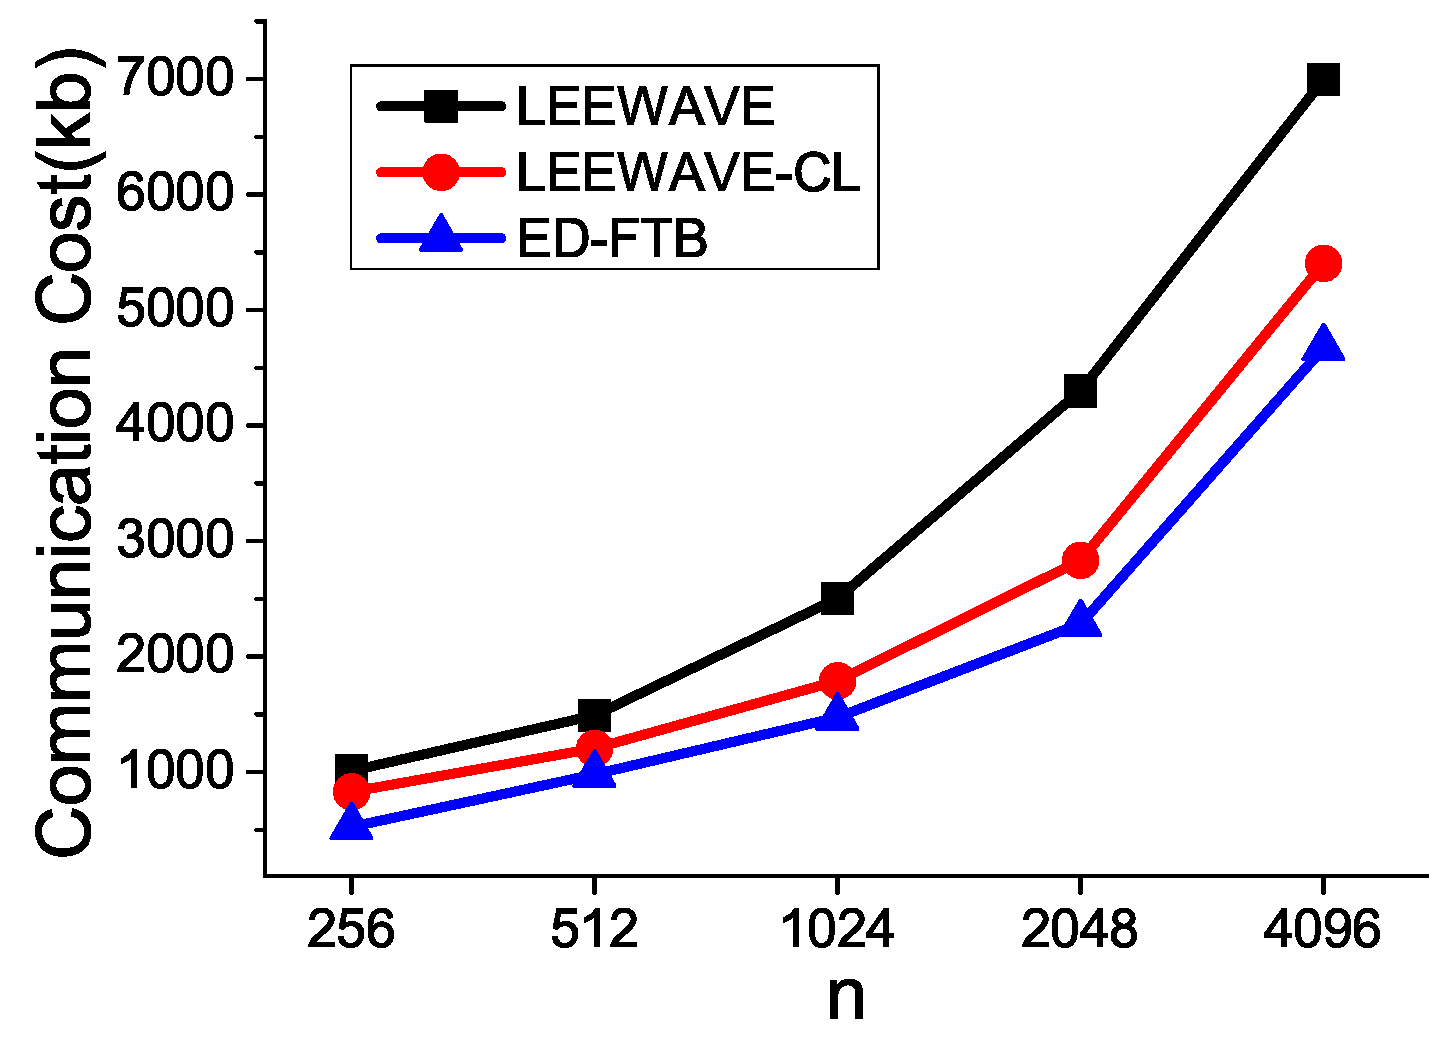
\includegraphics[width=2.7in]{Fig/chapter4/cmpk50.eps}
}
\subfigure[$k=100$]{
	\label{fig:costCmpk100}
	\includegraphics[width=2.7in]{Fig/chapter4/cmpk100.eps}
}
\caption{算法性能比较}
\label{fig:costCmp}
\end{figure}
接下来,我们将ED-FTB与LEEWAVE和LEEWAVE-CL进行通信性能比较。在该组实验中我们将轨迹长度$n$从256变化到$4,096$。图\ref{fig:costCmp}展示了当$k$取值为1,10和100下的结果。从该组图中我们可以看出,本文所提ED-FTB算法性能最好,LEEWAVE-CL其次,最差的是LEEWAVE。LEEWAVE-CL比LEEWAVE好的原因是它使用了本文所提下界进行剪枝。本文所提下界由于比LEEWAVE中的更加紧凑,因而剪枝效果更好。最终导致通信开销更低。而ED-FTB算法比LEEWAVE-CL好的原因是,本文采用的是在远程结点剪枝的策略,只需发送概要数据。而LEEWAVE和LEEWAVE-CL 均是采用在协调者结点剪枝的策略,除了发概要数据还要发送和接受其他额外数据。因而开销更高。最后,我们可以发现,随着轨迹长度$n$和$k$值的增加,EDD-FTB算法所节省的通信开销逐步增大。这进一步说明了本文算法的优越性。

\subsection{算法可扩展性}
\begin{figure} [t]
	\centering
	\subfigure[Running time in respect of $n$,$N$]{
		\label{fig:KLN}
		\includegraphics[width=2.7in]{Fig/chapter4/edtimeScalability.eps}		
	}
	\subfigure[Communication cost in respect of  $n$,$N$]{
		\label{fig:MN}
		\includegraphics[width=2.7in]{Fig/chapter4/edcommScalability.eps}
	}
	\caption{ED-FTB 算法可扩展性 {(T-Big数据集)}}
	\label{fig:EDScalability}
\end{figure}

 本小节我们将在\emph{T-Big}数据集上从时间和通信两个角度研究了ED-FTB算法的可扩展性。首先,考虑了轨迹数量$N$(即数据量大小)和轨迹长度$n$对可扩展性的影响。
在该组实验中,我们将$k$设置为1,$M$设置为$10,000$。我们将轨迹长度从$256$到$4096$进行指数级变化,同时将轨迹数量从10万到1百万进行线性增加。
  图\ref{fig:EDScalability}分别对这两个角度的结果进行了介绍,其中图\ref{fig:KLN}介绍了时间性能受$n$和$N$的影响(时间包系统初始化过程中对数据进行哈尔小波转换的开销)。我们可以看到对于任意长度的轨迹数据集,ED-FTB算法的运行时间都随着轨迹数据量的增加而线性增加。
  此外,随着轨迹长度的指数增加,算法的运行时间也指数增加,即运行时间与轨迹长度呈一定的线性关系。这一结果反映了由于ED-FTB的剪枝效果较好,导致迭代结束后,所剩候选数较少。即我们对ED-FTB算法时间复杂度分析部分的$N'$较少。结合以上两点,我们可以看出ED-FTB算法运行时间随着数据集的大小而线性变换,因此运行效率具有较好的可扩展性。

\section{本章小结}\label{sec-c4-conclusion}
本章节介绍了利用FTB框架在嵌入欧式距离下的具体实现算法ED-FTB。本章节,首先针对欧式距离,提出了基于哈尔小波系数的概要数据。接着,提出了基于哈尔小波系数的欧式距离上、下界。
该上、下界能够随着小波粒度的增加而逐渐变紧,这使得我们利用将该距离嵌入到FTB框架称为可能。为此,我们提出了ED-FTB算法以实现基于欧式距离的查询。在我们的查询算法中,我们引入了边计算下界边剪枝的查询优化措施,以提高执行效率。通过在真实数据集上进行的实验,表明所提方法剪枝效果由于现有方案,且具有较好的可扩展性。

\section*{本章证明附件}\label{sec-c4-Appendix}
\textbf{引理 \ref{theory:dis}. }{\em 给定两条轨迹${\cal Q}$ 和 ${\cal C}$,$H{\cal Q}$ 和 $H{\cal C}$分别表示${\cal Q}$ 和 ${\cal C}$经过哈尔小波变换后的系数序列。我们有如下结论:$SED({\cal Q},{\cal C})=SED(H{\cal Q},H{\cal C})$。}
\begin{proof}
	首先,根据$S_{i}({\cal Q}, {\cal C})$ 和 $SED_{i}({\cal Q}, {\cal C})$定义(定义\ref{eq:basic})我们有
	\allowdisplaybreaks
	\begin{eqnarray}
	&&	S_{i+1}({\cal Q}, {\cal C})=\sum\nolimits_{j=0}^{2^{i+1}-1}SED(\va_{i+1,j}^{\cal Q},\va_{i+1,j}^{\cal C}) \nonumber \\
	&=&SED(\va_{i+1,0}^{\cal Q},\va_{i+1,0}^{\cal C}) + SED(\va_{i+1,1}^{\cal Q},\va_{i+1,1}^{\cal C}) + \cdots + \nonumber \\
	&\,& SED(\va_{i+1,2^{i+1}-2}^{\cal Q},\va_{i+1,2^{i+1}-2}^{\cal C}) + 	SED(\va_{i+1,2^{i+1}-1}^{\cal Q},\va_{i+1,2^{i+1}-1}^{\cal C}) \nonumber \\
	&=&SED(\va_{i,0}^{\cal Q},\va_{i,0}^{\cal C})  +   SED(\vd_{i,0}^{\cal Q}, \vd_{i,0}^{\cal C})   + \cdots+\nonumber \\
	&\,& SED(\va_{i,2^{i}-1}^{\cal Q},\va_{i,2^{i}-1}^{\cal C})  +   SED(\vd_{i,2^{i}-1}^{\cal Q}, \vd_{i,2^{i}-1}^{\cal C})  \nonumber   \nonumber \\
	&=& \sum\nolimits_{j=0}^{2^i-1}SED(\va_{i,j}^{\cal Q}, \va_{i,j}^{\cal C})+ \sum\nolimits_{j=0}^{2^i-1}SED(\vd_{i,j}^{\cal Q}, \vd_{i,j}^{\cal C})\nonumber \\
	&=&S_{i}({\cal Q}, {\cal C})+SED_{i}({\cal Q},{\cal C})
	\end{eqnarray}
	\allowdisplaybreaks[4]
根据如上公式,对于叶子层结点,我们有:
	\begin{eqnarray} \label{eq:prove1L}
	S_{L}({\cal Q},{\cal C})&=&S_{0}({\cal Q},{\cal C})+ \sum\nolimits_{i=0}^{L-1}{SED_{i}({\cal Q},{\cal C})} \nonumber \\
	&=& SED(H{\cal Q},H{\cal C})
	\end{eqnarray}
	此外,第$L$层为叶子节点层,包含了轨迹的原始信息。所以我们又有$SED({\cal Q},{\cal C}) = S_{L}({\cal Q},{\cal C})$。此时结合公式\ref{eq:prove1L}
	我们得到 $SED({\cal Q},{\cal C})=SED(H{\cal Q},H{\cal C})$。原问题得证。
\end{proof}

\textbf{定理 \ref{theory:lower}. }{\em $HLB$会随着粒度的概要数据粒度的增加而逐渐上升,即$HLB_{l} \le HLB_{l+1}$。}
至此,我们根据哈尔小波变换得到原始轨迹不同粒度概要数据,并根据概要数据提出了欧式距离的上、下界。


\begin{proof}\label{proof:p2}
	我们的策略是证明 $HLB_{l+1}- HLB_{l}\ge 0$。我们首先将其左半部分展开:
	\begin{eqnarray}\label{eq:minus}
HLB_{l+1}- HLB_{l}= SED_{l+1}({\cal Q},{\cal C}) - \sum\nolimits_{j=0}^{2^{l+1}-1}(||\vd_{l+1,j}^{\cal Q}||^2  + ||\vd_{l+1,j}^{\cal C}||^2)+\nonumber\\
 2(\sqrt{\sum_{i=l+1}^{L -1}\sum_{j=0}^{2^i-1}||\vd_{i,j}^{\cal Q}||^2} \cdot \sqrt{\sum_{i=l+1}^{L -1}\sum_{j=0}^{2^i-1}||\vd_{i,j}^{\cal C}||^2} -\sqrt{\sum_{i=l+2}^{L -1}\sum_{j=0}^{2^i-1}||\vd_{i,j}^{\cal Q}||^2} \cdot \sqrt{\sum_{i=l+2}^{L -1}\sum_{j=0}^{2^i-1}||\vd_{i,j}^{\cal C}||^2})\nonumber
	\end{eqnarray}	
	接着, 我们将$SED_{l+1}({\cal Q},{\cal C})$ 展开得到$SED_{l+1}({\cal Q},{\cal C})=\sum_{j=0}^{2^{l+1}-1}{(||\vd_{l+1,j}^{\cal Q}||^2+||\vd_{l+1,j}^{\cal C}||^2}-2 \vd_{l+1,j}^{\cal Q} \bigcdot \vd_{l+1,j}^{\cal C})$。我们的问题变为证明如下不等式成立。
	\begin{eqnarray}\label{eq:InEq}
	\sum_{j=0}^{2^{l+1}-1}\vd_{l+1,j}^{\cal Q} \bigcdot \vd_{l+1,j}^{\cal C} &\le& \sqrt{\sum_{i=l+1}^{L-1}\sum_{j=0}^{2^i-1}||\vd_{i,j}^{\cal Q}||^2} \cdot \sqrt{\sum_{i=l+1}^{L-1}\sum_{j=0}^{2^i-1}||\vd_{i,j}^{\cal C}||^2} \nonumber\\
&\quad&	-	\sqrt{\sum_{i=l+2}^{L-1}\sum_{j=0}^{2^i-1}||\vd_{i,j}^{\cal Q}||^2} \cdot \sqrt{\sum_{i=l+2}^{L-1}\sum_{j=0}^{2^i-1}||\vd_{i,j}^{\cal C}||^2} 
	\end{eqnarray}	
	对于不等式 \ref{eq:InEq}的左半部分我们有
	$\sum_{j=0}^{2^{l+1}-1}\vd_{l+1,j}^{\cal Q}\bigcdot \vd_{l+1,j}^{\cal C} \le
	\sqrt{\sum_{j=0}^{2^{l+1}-1}||\vd_{l+1,j}^{\cal Q}||^2} \cdot \sqrt{\sum_{j=0}^{2^{l+1}-1}||\vd_{l+1,j}^{\cal C}||^2}$。
	所以我们的目标变为证明
	$\sqrt{\sum_{j=0}^{2^{l+1}-1}||\vd_{l+1,j}^{\cal Q}||^2} \cdot \sqrt{\sum_{j=0}^{2^{l+1}-1}||\vd_{l+1,j}^{\cal C}||^2}$
	小于不等式\ref{eq:InEq}的右半部分。
	为方便表示,我们令$x= \sum_{j=0}^{2^{l+1}-1}||\vd_{l+1,j}^{\cal Q}||^2$,$y=\sum_{j=0}^{2^{l+1}-1}||\vd_{l+1,j}^{\cal C}||^2$,$\alpha = \sum_{i=l+2}^{L-1}\sum_{j=0}^{2^l-1}||\vd_{i,j}^{\cal Q}||^2$,$\beta =  \sum_{i=l+2}^{L-1}\sum_{j=0}^{2^l-1}||\vd_{i,j}^{\cal C}||^2$。
	则不等于\ref{eq:InEq}等价于:
	\begin{eqnarray}\label{eq:sim}
	\sqrt{x \cdot y} + \sqrt{\alpha \cdot \beta} \le \sqrt{(\alpha+x) \cdot (\beta+y)}
	\end{eqnarray}	
	我们将如上不等式两边平方得到如下不等式:
	\begin{eqnarray}\label{eq:final}
	2\sqrt{x\cdot y \cdot \alpha \cdot \beta} \le \alpha \cdot y+\beta\cdot x
	\end{eqnarray}	
	根据算数-几何平均不等式,我们得不等式\ref{eq:final} 成立。原问题得证。
\end{proof}

%% Property 2
\textbf{定理 \ref{theory:upper}. }{\em $HUB$会随着粒度的概要数据粒度的增加而逐渐下降,即$HUB_{l+1} \le HLB_{l}$。}
\begin{proof}
	我们的策略是证明 $HUB_{l+1}- HUB_{l}\le 0$。我们首先将其左半部分展开:
	\begin{eqnarray}\label{eq:minusupper}
	HUB_{l+1}- HUB_{l}= SED_{l+1}({\cal Q},{\cal C}) - \sum\nolimits_{j=0}^{2^{l+1}-1}(||\vd_{l+1,j}^{\cal Q}||^2  + ||\vd_{l+1,j}^{\cal C}||^2) -\nonumber\\
	2(\sqrt{\sum_{i=l+1}^{L -1}\sum_{j=0}^{2^i-1}||\vd_{i,j}^{\cal Q}||^2} \cdot \sqrt{\sum_{i=l+1}^{L -1}\sum_{j=0}^{2^i-1}||\vd_{i,j}^{\cal C}||^2} -\sqrt{\sum_{i=l+2}^{L -1}\sum_{j=0}^{2^i-1}||\vd_{i,j}^{\cal Q}||^2} \cdot \sqrt{\sum_{i=l+2}^{L -1}\sum_{j=0}^{2^i-1}||\vd_{i,j}^{\cal C}||^2})\nonumber
	\end{eqnarray}	
		接着, 我们将$SED_{l+1}({\cal Q},{\cal C})$ 展开得到$SED_{l+1}({\cal Q},{\cal C})=\sum_{j=0}^{2^{l+1}-1}{(||\vd_{l+1,j}^{\cal Q}||^2+||\vd_{l+1,j}^{\cal C}||^2}-2 \vd_{l+1,j}^{\cal Q} \bigcdot \vd_{l+1,j}^{\cal C})$。我们的问题变为证明如下不等式成立。
	\begin{eqnarray}\label{eq:InEqUB}
	\sum_{j=0}^{2^{l+1}-1}\vd_{l+1,j}^{\cal Q} \bigcdot \vd_{l+1,j}^{\cal C} &\ge&
	\sqrt{\sum_{i=l+2}^{L-1}\sum_{j=0}^{2^i-1}||\vd_{i,j}^{\cal Q}||^2} \cdot \sqrt{\sum_{i=l+2}^{L-1}\sum_{j=0}^{2^i-1}||\vd_{i,j}^{\cal C}||^2} \nonumber\\
	&\quad&	-		 \sqrt{\sum_{i=l+1}^{L-1}\sum_{j=0}^{2^i-1}||\vd_{i,j}^{\cal Q}||^2} \cdot \sqrt{\sum_{i=l+1}^{L-1}\sum_{j=0}^{2^i-1}||\vd_{i,j}^{\cal C}||^2} 
	\end{eqnarray}	
	由于	$\sum_{j=0}^{2^{l+1}-1}\vd_{l+1,j}^{\cal Q}\bigcdot \vd_{l+1,j}^{\cal C} \ge
-	\sqrt{\sum_{j=0}^{2^{l+1}-1}||\vd_{l+1,j}^{\cal Q}||^2} \cdot \sqrt{\sum_{j=0}^{2^{l+1}-1}||\vd_{l+1,j}^{\cal C}||^2}$,所以我们的问题变为证明$-\sqrt{\sum_{j=0}^{2^{l+1}-1}||\vd_{l+1,j}^{\cal Q}||^2} \cdot \sqrt{\sum_{j=0}^{2^{l+1}-1}||\vd_{l+1,j}^{\cal C}||^2} $大于公式\ref{eq:InEqUB}右半部分。与定理\ref{theory:lower}证明类似,我们令$x= \sum_{j=0}^{2^{l+1}-1}||\vd_{l+1,j}^{\cal Q}||^2$,$y=\sum_{j=0}^{2^{l+1}-1}||\vd_{l+1,j}^{\cal C}||^2$,$\alpha = \sum_{i=l+2}^{L-1}\sum_{j=0}^{2^l-1}||\vd_{i,j}^{\cal Q}||^2$,$\beta =  \sum_{i=l+2}^{L-1}\sum_{j=0}^{2^l-1}||\vd_{i,j}^{\cal C}||^2$。
	则不等于\ref{eq:InEqUB}等价于:
	\begin{eqnarray}\label{eq:simUB}
	- \sqrt{x \cdot y} \ge  \sqrt{\alpha \cdot \beta}  -  \sqrt{(\alpha+x) \cdot (\beta+y)} 
% \sqrt{(\alpha+x) \cdot (\beta+y)} \le 	\sqrt{x \cdot y} + \sqrt{\alpha \cdot \beta} 
	\end{eqnarray}	
	不等式经过变换可得到不等式\ref{eq:sim}。因此可得不等式\ref{eq:InEqUB}成立,原问题得证。
\end{proof}


\clearpage
\phantom{s}
\clearpage